%master file for final report
%this will contain \input for each of the sections, and all the general formatting.
%this will need editing if additional packages are used

\documentclass[twoside,12pt]{article}
%\usepackage{helvet}
%\renewcommand{\familydefault}{\sfdefault}
%\usepackage[T1]{fontenc}

\renewcommand{\baselinestretch}{1.5}
\usepackage[
    backend=bibtex,
    citestyle=numeric,
    doi=true,
    eprint=false
]{biblatex}
\addbibresource{bibliography.bib} %for references

%%% PACKAGES
\usepackage{geometry} % to change the page dimensions
\geometry{a4paper} % or letterpaper (US) or a5paper or....
 \geometry{margin=22mm} % for example, change the margins to 2 inches all round
% \geometry{landscape} % set up the page for landscape
%   read geometry.pdf for detailed page layout information

\usepackage{graphicx} % support the \includegraphics command and options
%\usepackage{wrapfig}
\usepackage{fixltx2e} % type subscripts in text not in equation mode
\usepackage{subcaption}
\usepackage{float}    % allows to position floats with [H]

% \usepackage[parfill]{parskip} % Activate to begin paragraphs with an empty line rather than an indent
\usepackage{amsmath}
\usepackage{amsfonts}

\usepackage{booktabs} % for much better looking tables
\usepackage{array} % for better arrays (eg matrices) in maths
%\usepackage[binary-units]{siunitx} % for scientific notation and SI units, bytes
%\usepackage{paralist} % very flexible & customisable lists (eg. enumerate/itemize, etc.)
\usepackage{verbatim} % adds environment for commenting out blocks of text & for better verbatim
\usepackage{subfig} % make it possible to include more than one captioned figure/table in a single float
% These packages are all incorporated in the memoir class to one degree or another...

%%% HEADERS & FOOTERS
\usepackage{fancyhdr} % This should be set AFTER setting up the page geometry
\fancypagestyle{StephenFoot}{%
\renewcommand{\headrulewidth}{0pt}
\lhead{}\chead{}\rhead{}
\fancyfoot[LE,RO]{Stephen Lilico}\cfoot{\thepage}
}

%\usepackage{authblk} %package to allow us to include our institute nicely

\usepackage{algpseudocode} %pseudocode
%\algrenewcommand{\algorithmiccomment}[1]{\hskip5em\%#1}

\algblockx[WithP]{WithP}{EndP}%withprobability command
	[1][oops?]{\textbf{with probability #1} :}
	{\textbf{end}}
\algcblockx[Pelse]{WithP}{ElseP}{EndP}
	{\textbf{else}}
	{\textbf{end}}
	
\usepackage{tikz} %for graphics made in Latex (so flowcharts/mindmaps/simple diagrams)
    \usetikzlibrary{trees, positioning,arrows,graphs,shapes,shadows,fit}
\usepackage{pgfplots} %for graph plotting
%\usepgfplotslibrary{external} 
%\tikzexternalize %externalises processing to save memory
\pgfplotsset{
    mark one*/.style={
        scatter,
        scatter src=x,
        scatter/@pre marker code/.code={
            \pgfmathtruncatemacro\usemark{
               \coordindex == #1
            }
            \ifnum\usemark=0
                \pgfplotsset{mark=none}
            \fi
        },
        scatter/@post marker code/.code={}
    }
}
\pgfplotsset{
  colormap/closeto0/.style={
    colormap={closeto0}{
    rgb255(0cm)=(0,255,0);
    rgb255(0.1cm)=(0,160,120); 
    rgb255(0.5cm)=(0,0,255); 
    rgb255(2cm)=(255,0,0); 
    }
  }
 }


\pgfplotsset{
  colormap/viridis/.style={
    colormap={viridis}{
      rgb=(0.26700401,  0.00487433,  0.32941519)
      rgb=(0.26851048,  0.00960483,  0.33542652)
      rgb=(0.26994384,  0.01462494,  0.34137895)
      rgb=(0.27130489,  0.01994186,  0.34726862)
      rgb=(0.27259384,  0.02556309,  0.35309303)
      rgb=(0.27380934,  0.03149748,  0.35885256)
      rgb=(0.27495242,  0.03775181,  0.36454323)
      rgb=(0.27602238,  0.04416723,  0.37016418)
      rgb=(0.2770184 ,  0.05034437,  0.37571452)
      rgb=(0.27794143,  0.05632444,  0.38119074)
      rgb=(0.27879067,  0.06214536,  0.38659204)
      rgb=(0.2795655 ,  0.06783587,  0.39191723)
      rgb=(0.28026658,  0.07341724,  0.39716349)
      rgb=(0.28089358,  0.07890703,  0.40232944)
      rgb=(0.28144581,  0.0843197 ,  0.40741404)
      rgb=(0.28192358,  0.08966622,  0.41241521)
      rgb=(0.28232739,  0.09495545,  0.41733086)
      rgb=(0.28265633,  0.10019576,  0.42216032)
      rgb=(0.28291049,  0.10539345,  0.42690202)
      rgb=(0.28309095,  0.11055307,  0.43155375)
      rgb=(0.28319704,  0.11567966,  0.43611482)
      rgb=(0.28322882,  0.12077701,  0.44058404)
      rgb=(0.28318684,  0.12584799,  0.44496   )
      rgb=(0.283072  ,  0.13089477,  0.44924127)
      rgb=(0.28288389,  0.13592005,  0.45342734)
      rgb=(0.28262297,  0.14092556,  0.45751726)
      rgb=(0.28229037,  0.14591233,  0.46150995)
      rgb=(0.28188676,  0.15088147,  0.46540474)
      rgb=(0.28141228,  0.15583425,  0.46920128)
      rgb=(0.28086773,  0.16077132,  0.47289909)
      rgb=(0.28025468,  0.16569272,  0.47649762)
      rgb=(0.27957399,  0.17059884,  0.47999675)
      rgb=(0.27882618,  0.1754902 ,  0.48339654)
      rgb=(0.27801236,  0.18036684,  0.48669702)
      rgb=(0.27713437,  0.18522836,  0.48989831)
      rgb=(0.27619376,  0.19007447,  0.49300074)
      rgb=(0.27519116,  0.1949054 ,  0.49600488)
      rgb=(0.27412802,  0.19972086,  0.49891131)
      rgb=(0.27300596,  0.20452049,  0.50172076)
      rgb=(0.27182812,  0.20930306,  0.50443413)
      rgb=(0.27059473,  0.21406899,  0.50705243)
      rgb=(0.26930756,  0.21881782,  0.50957678)
      rgb=(0.26796846,  0.22354911,  0.5120084 )
      rgb=(0.26657984,  0.2282621 ,  0.5143487 )
      rgb=(0.2651445 ,  0.23295593,  0.5165993 )
      rgb=(0.2636632 ,  0.23763078,  0.51876163)
      rgb=(0.26213801,  0.24228619,  0.52083736)
      rgb=(0.26057103,  0.2469217 ,  0.52282822)
      rgb=(0.25896451,  0.25153685,  0.52473609)
      rgb=(0.25732244,  0.2561304 ,  0.52656332)
      rgb=(0.25564519,  0.26070284,  0.52831152)
      rgb=(0.25393498,  0.26525384,  0.52998273)
      rgb=(0.25219404,  0.26978306,  0.53157905)
      rgb=(0.25042462,  0.27429024,  0.53310261)
      rgb=(0.24862899,  0.27877509,  0.53455561)
      rgb=(0.2468114 ,  0.28323662,  0.53594093)
      rgb=(0.24497208,  0.28767547,  0.53726018)
      rgb=(0.24311324,  0.29209154,  0.53851561)
      rgb=(0.24123708,  0.29648471,  0.53970946)
      rgb=(0.23934575,  0.30085494,  0.54084398)
      rgb=(0.23744138,  0.30520222,  0.5419214 )
      rgb=(0.23552606,  0.30952657,  0.54294396)
      rgb=(0.23360277,  0.31382773,  0.54391424)
      rgb=(0.2316735 ,  0.3181058 ,  0.54483444)
      rgb=(0.22973926,  0.32236127,  0.54570633)
      rgb=(0.22780192,  0.32659432,  0.546532  )
      rgb=(0.2258633 ,  0.33080515,  0.54731353)
      rgb=(0.22392515,  0.334994  ,  0.54805291)
      rgb=(0.22198915,  0.33916114,  0.54875211)
      rgb=(0.22005691,  0.34330688,  0.54941304)
      rgb=(0.21812995,  0.34743154,  0.55003755)
      rgb=(0.21620971,  0.35153548,  0.55062743)
      rgb=(0.21429757,  0.35561907,  0.5511844 )
      rgb=(0.21239477,  0.35968273,  0.55171011)
      rgb=(0.2105031 ,  0.36372671,  0.55220646)
      rgb=(0.20862342,  0.36775151,  0.55267486)
      rgb=(0.20675628,  0.37175775,  0.55311653)
      rgb=(0.20490257,  0.37574589,  0.55353282)
      rgb=(0.20306309,  0.37971644,  0.55392505)
      rgb=(0.20123854,  0.38366989,  0.55429441)
      rgb=(0.1994295 ,  0.38760678,  0.55464205)
      rgb=(0.1976365 ,  0.39152762,  0.55496905)
      rgb=(0.19585993,  0.39543297,  0.55527637)
      rgb=(0.19410009,  0.39932336,  0.55556494)
      rgb=(0.19235719,  0.40319934,  0.55583559)
      rgb=(0.19063135,  0.40706148,  0.55608907)
      rgb=(0.18892259,  0.41091033,  0.55632606)
      rgb=(0.18723083,  0.41474645,  0.55654717)
      rgb=(0.18555593,  0.4185704 ,  0.55675292)
      rgb=(0.18389763,  0.42238275,  0.55694377)
      rgb=(0.18225561,  0.42618405,  0.5571201 )
      rgb=(0.18062949,  0.42997486,  0.55728221)
      rgb=(0.17901879,  0.43375572,  0.55743035)
      rgb=(0.17742298,  0.4375272 ,  0.55756466)
      rgb=(0.17584148,  0.44128981,  0.55768526)
      rgb=(0.17427363,  0.4450441 ,  0.55779216)
      rgb=(0.17271876,  0.4487906 ,  0.55788532)
      rgb=(0.17117615,  0.4525298 ,  0.55796464)
      rgb=(0.16964573,  0.45626209,  0.55803034)
      rgb=(0.16812641,  0.45998802,  0.55808199)
      rgb=(0.1666171 ,  0.46370813,  0.55811913)
      rgb=(0.16511703,  0.4674229 ,  0.55814141)
      rgb=(0.16362543,  0.47113278,  0.55814842)
      rgb=(0.16214155,  0.47483821,  0.55813967)
      rgb=(0.16066467,  0.47853961,  0.55811466)
      rgb=(0.15919413,  0.4822374 ,  0.5580728 )
      rgb=(0.15772933,  0.48593197,  0.55801347)
      rgb=(0.15626973,  0.4896237 ,  0.557936  )
      rgb=(0.15481488,  0.49331293,  0.55783967)
      rgb=(0.15336445,  0.49700003,  0.55772371)
      rgb=(0.1519182 ,  0.50068529,  0.55758733)
      rgb=(0.15047605,  0.50436904,  0.55742968)
      rgb=(0.14903918,  0.50805136,  0.5572505 )
      rgb=(0.14760731,  0.51173263,  0.55704861)
      rgb=(0.14618026,  0.51541316,  0.55682271)
      rgb=(0.14475863,  0.51909319,  0.55657181)
      rgb=(0.14334327,  0.52277292,  0.55629491)
      rgb=(0.14193527,  0.52645254,  0.55599097)
      rgb=(0.14053599,  0.53013219,  0.55565893)
      rgb=(0.13914708,  0.53381201,  0.55529773)
      rgb=(0.13777048,  0.53749213,  0.55490625)
      rgb=(0.1364085 ,  0.54117264,  0.55448339)
      rgb=(0.13506561,  0.54485335,  0.55402906)
      rgb=(0.13374299,  0.54853458,  0.55354108)
      rgb=(0.13244401,  0.55221637,  0.55301828)
      rgb=(0.13117249,  0.55589872,  0.55245948)
      rgb=(0.1299327 ,  0.55958162,  0.55186354)
      rgb=(0.12872938,  0.56326503,  0.55122927)
      rgb=(0.12756771,  0.56694891,  0.55055551)
      rgb=(0.12645338,  0.57063316,  0.5498411 )
      rgb=(0.12539383,  0.57431754,  0.54908564)
      rgb=(0.12439474,  0.57800205,  0.5482874 )
      rgb=(0.12346281,  0.58168661,  0.54744498)
      rgb=(0.12260562,  0.58537105,  0.54655722)
      rgb=(0.12183122,  0.58905521,  0.54562298)
      rgb=(0.12114807,  0.59273889,  0.54464114)
      rgb=(0.12056501,  0.59642187,  0.54361058)
      rgb=(0.12009154,  0.60010387,  0.54253043)
      rgb=(0.11973756,  0.60378459,  0.54139999)
      rgb=(0.11951163,  0.60746388,  0.54021751)
      rgb=(0.11942341,  0.61114146,  0.53898192)
      rgb=(0.11948255,  0.61481702,  0.53769219)
      rgb=(0.11969858,  0.61849025,  0.53634733)
      rgb=(0.12008079,  0.62216081,  0.53494633)
      rgb=(0.12063824,  0.62582833,  0.53348834)
      rgb=(0.12137972,  0.62949242,  0.53197275)
      rgb=(0.12231244,  0.63315277,  0.53039808)
      rgb=(0.12344358,  0.63680899,  0.52876343)
      rgb=(0.12477953,  0.64046069,  0.52706792)
      rgb=(0.12632581,  0.64410744,  0.52531069)
      rgb=(0.12808703,  0.64774881,  0.52349092)
      rgb=(0.13006688,  0.65138436,  0.52160791)
      rgb=(0.13226797,  0.65501363,  0.51966086)
      rgb=(0.13469183,  0.65863619,  0.5176488 )
      rgb=(0.13733921,  0.66225157,  0.51557101)
      rgb=(0.14020991,  0.66585927,  0.5134268 )
      rgb=(0.14330291,  0.66945881,  0.51121549)
      rgb=(0.1466164 ,  0.67304968,  0.50893644)
      rgb=(0.15014782,  0.67663139,  0.5065889 )
      rgb=(0.15389405,  0.68020343,  0.50417217)
      rgb=(0.15785146,  0.68376525,  0.50168574)
      rgb=(0.16201598,  0.68731632,  0.49912906)
      rgb=(0.1663832 ,  0.69085611,  0.49650163)
      rgb=(0.1709484 ,  0.69438405,  0.49380294)
      rgb=(0.17570671,  0.6978996 ,  0.49103252)
      rgb=(0.18065314,  0.70140222,  0.48818938)
      rgb=(0.18578266,  0.70489133,  0.48527326)
      rgb=(0.19109018,  0.70836635,  0.48228395)
      rgb=(0.19657063,  0.71182668,  0.47922108)
      rgb=(0.20221902,  0.71527175,  0.47608431)
      rgb=(0.20803045,  0.71870095,  0.4728733 )
      rgb=(0.21400015,  0.72211371,  0.46958774)
      rgb=(0.22012381,  0.72550945,  0.46622638)
      rgb=(0.2263969 ,  0.72888753,  0.46278934)
      rgb=(0.23281498,  0.73224735,  0.45927675)
      rgb=(0.2393739 ,  0.73558828,  0.45568838)
      rgb=(0.24606968,  0.73890972,  0.45202405)
      rgb=(0.25289851,  0.74221104,  0.44828355)
      rgb=(0.25985676,  0.74549162,  0.44446673)
      rgb=(0.26694127,  0.74875084,  0.44057284)
      rgb=(0.27414922,  0.75198807,  0.4366009 )
      rgb=(0.28147681,  0.75520266,  0.43255207)
      rgb=(0.28892102,  0.75839399,  0.42842626)
      rgb=(0.29647899,  0.76156142,  0.42422341)
      rgb=(0.30414796,  0.76470433,  0.41994346)
      rgb=(0.31192534,  0.76782207,  0.41558638)
      rgb=(0.3198086 ,  0.77091403,  0.41115215)
      rgb=(0.3277958 ,  0.77397953,  0.40664011)
      rgb=(0.33588539,  0.7770179 ,  0.40204917)
      rgb=(0.34407411,  0.78002855,  0.39738103)
      rgb=(0.35235985,  0.78301086,  0.39263579)
      rgb=(0.36074053,  0.78596419,  0.38781353)
      rgb=(0.3692142 ,  0.78888793,  0.38291438)
      rgb=(0.37777892,  0.79178146,  0.3779385 )
      rgb=(0.38643282,  0.79464415,  0.37288606)
      rgb=(0.39517408,  0.79747541,  0.36775726)
      rgb=(0.40400101,  0.80027461,  0.36255223)
      rgb=(0.4129135 ,  0.80304099,  0.35726893)
      rgb=(0.42190813,  0.80577412,  0.35191009)
      rgb=(0.43098317,  0.80847343,  0.34647607)
      rgb=(0.44013691,  0.81113836,  0.3409673 )
      rgb=(0.44936763,  0.81376835,  0.33538426)
      rgb=(0.45867362,  0.81636288,  0.32972749)
      rgb=(0.46805314,  0.81892143,  0.32399761)
      rgb=(0.47750446,  0.82144351,  0.31819529)
      rgb=(0.4870258 ,  0.82392862,  0.31232133)
      rgb=(0.49661536,  0.82637633,  0.30637661)
      rgb=(0.5062713 ,  0.82878621,  0.30036211)
      rgb=(0.51599182,  0.83115784,  0.29427888)
      rgb=(0.52577622,  0.83349064,  0.2881265 )
      rgb=(0.5356211 ,  0.83578452,  0.28190832)
      rgb=(0.5455244 ,  0.83803918,  0.27562602)
      rgb=(0.55548397,  0.84025437,  0.26928147)
      rgb=(0.5654976 ,  0.8424299 ,  0.26287683)
      rgb=(0.57556297,  0.84456561,  0.25641457)
      rgb=(0.58567772,  0.84666139,  0.24989748)
      rgb=(0.59583934,  0.84871722,  0.24332878)
      rgb=(0.60604528,  0.8507331 ,  0.23671214)
      rgb=(0.61629283,  0.85270912,  0.23005179)
      rgb=(0.62657923,  0.85464543,  0.22335258)
      rgb=(0.63690157,  0.85654226,  0.21662012)
      rgb=(0.64725685,  0.85839991,  0.20986086)
      rgb=(0.65764197,  0.86021878,  0.20308229)
      rgb=(0.66805369,  0.86199932,  0.19629307)
      rgb=(0.67848868,  0.86374211,  0.18950326)
      rgb=(0.68894351,  0.86544779,  0.18272455)
      rgb=(0.69941463,  0.86711711,  0.17597055)
      rgb=(0.70989842,  0.86875092,  0.16925712)
      rgb=(0.72039115,  0.87035015,  0.16260273)
      rgb=(0.73088902,  0.87191584,  0.15602894)
      rgb=(0.74138803,  0.87344918,  0.14956101)
      rgb=(0.75188414,  0.87495143,  0.14322828)
      rgb=(0.76237342,  0.87642392,  0.13706449)
      rgb=(0.77285183,  0.87786808,  0.13110864)
      rgb=(0.78331535,  0.87928545,  0.12540538)
      rgb=(0.79375994,  0.88067763,  0.12000532)
      rgb=(0.80418159,  0.88204632,  0.11496505)
      rgb=(0.81457634,  0.88339329,  0.11034678)
      rgb=(0.82494028,  0.88472036,  0.10621724)
      rgb=(0.83526959,  0.88602943,  0.1026459 )
      rgb=(0.84556056,  0.88732243,  0.09970219)
      rgb=(0.8558096 ,  0.88860134,  0.09745186)
      rgb=(0.86601325,  0.88986815,  0.09595277)
      rgb=(0.87616824,  0.89112487,  0.09525046)
      rgb=(0.88627146,  0.89237353,  0.09537439)
      rgb=(0.89632002,  0.89361614,  0.09633538)
      rgb=(0.90631121,  0.89485467,  0.09812496)
      rgb=(0.91624212,  0.89609127,  0.1007168 )
      rgb=(0.92610579,  0.89732977,  0.10407067)
      rgb=(0.93590444,  0.8985704 ,  0.10813094)
      rgb=(0.94563626,  0.899815  ,  0.11283773)
      rgb=(0.95529972,  0.90106534,  0.11812832)
      rgb=(0.96489353,  0.90232311,  0.12394051)
      rgb=(0.97441665,  0.90358991,  0.13021494)
      rgb=(0.98386829,  0.90486726,  0.13689671)
      rgb=(0.99324789,  0.90615657,  0.1439362 )
    }
  }
}


\usepackage{rotating} %to rotate a table
\usepackage{setspace}

\usepackage{abstract} %allows us to have an abstract formatted as such
   \renewcommand{\abstractnamefont}{\normalfont\large\bfseries}
   \renewcommand{\abstracttextfont}{\normalfont\normalsize}
   \setlength{\abstitleskip}{-0.8em}
   \newcommand{\tabitem}{~~\llap{\textbullet}~~}

\usepackage{wrapfig} %allows wrapping text around figure
\usepackage{amsmath} %advanced mathematical environment
\usepackage{pdfpages}
%to allow me to have something in the ToC but not have a title
\newcommand\invisiblesection[1]{%
  \refstepcounter{section}%
  \addcontentsline{toc}{section}{\protect\numberline{\thesection}#1}%
  \sectionmark{#1}}


\title{Report for 4YP Project: \\ Gaming AI}
\author{Stephen Lilico}

\begin{document}
  \maketitle
  
  \newpage
  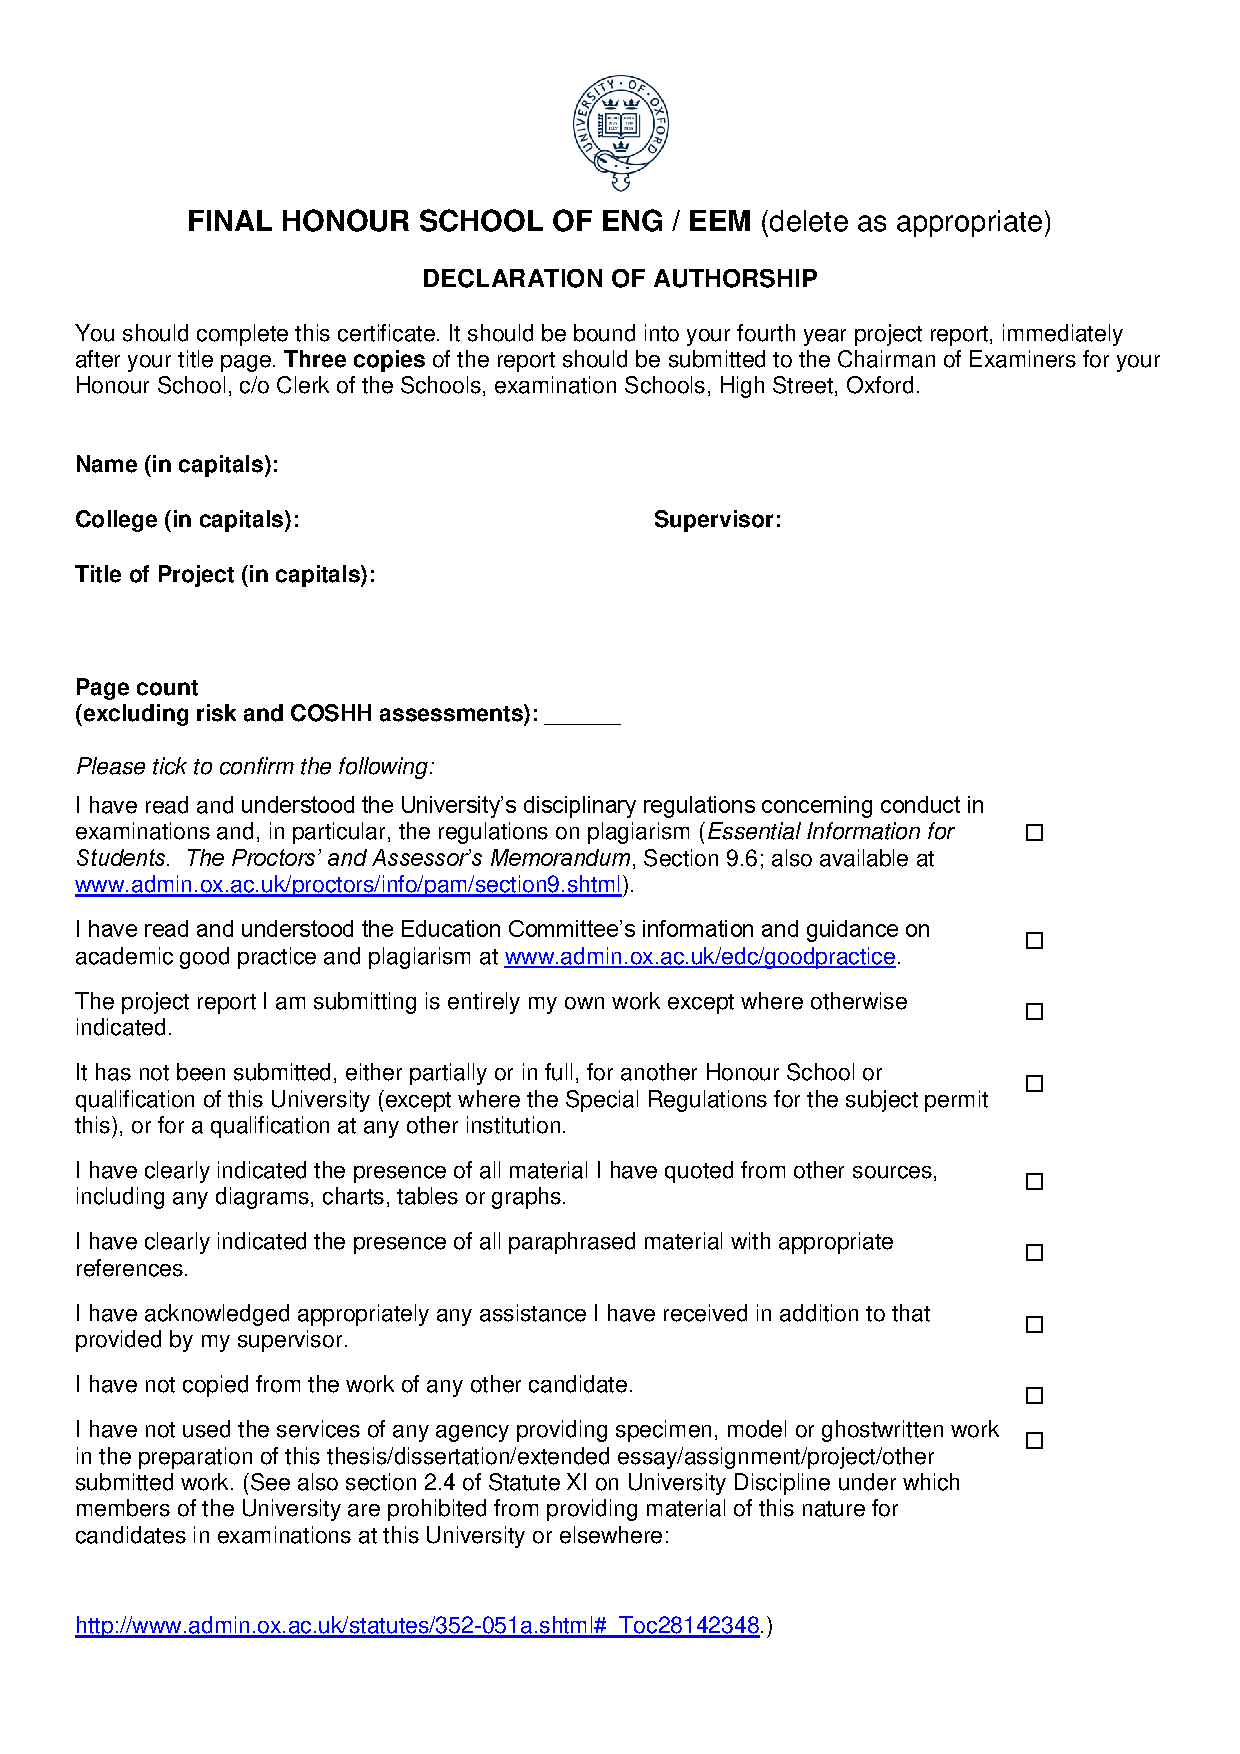
\includepdf[pages=-]{Declaration_of_Authorship.pdf}
  \newpage
  %abstract
  \begin{abstract}
	Recent advances in reinforcement learning have shown it to be possible to use it to train neural networks for complex tasks. This report sets out to see if these techniques can be used to leverage the significant power of neural networks to implicitly discover powerful policies, in particular to the cases of playing a trading card game and finding the optimum value of an unknown function that is expensive to compute.
	
	%this will need rewriting
  \end{abstract}
  \tableofcontents 
   %introduction to the projects overall goals
  \section{Introduction}
  %what is this about
This report details the research the author did in the academic year 2015-16 concerning reinforcement learning and it's uses. The initial goal of the project was to develop an AI that would be able to play some form of video game using reinforcement learning and neural networks as function approximators. However, halfway through an potentially more fruitful line of research opened up, and the project was redirected to consider how to develop a reinforcement learning agent that can optimize any given function in a minimum of steps.

The primary results of this research are an exploration of the limits of current technology to parse complex situations and produce meaningful behavior, and in particular the limitations of using Reinforcement learning to train neural networks for control in such tasks.

\subsection{Context}
  %why do we care?
Beyond immediate applications in terms of producing better quality AI for video games themselves, such research is really helpful to 


\subsection{Objectives}
%what are we trying to do

\subsection{Report structure}

%how the rest of the report flows
  %literature review needs to go here
  \section{Literature Review}
%this will detail all the prior work we're building on here.
%we can say more here - both more detail and more background if needed
This section details the mathematical framework and previous research on which this project was based.

\subsection{Artificial Neural Networks}
This project uses artificial neural networks for the approximation of various functions within the agent. Artificial neural networks can be considered to be general function approximators - they learn a non-linear mapping between their inputs and outputs, the complexity of which is dependant on the hyper parameters and structure of the network.

At their most basic, a neural network consists of layers of ``neurons''. Each neuron takes a linear sum of their inputs (often the output of all the neurons in the previous layer, plus an optional bias term, but not always), then applies a non-linear ``activation function'' to that.  So the output of the jth neuron in the layer could be written as:
\begin{equation}
O_j = f\big( \sum_i (w_{ji}I_i)\big)
\end{equation} where $f(x)$ is the non-linear activation function - for example the sigmoid function, $\frac{1}{1+ \text{e}^{-x}}$.  $w_ij$ are model parameters that are learned. The non-linearity allows multiple consecutive layers to add further expressiveness to the function, and the choice of what non-linearity is used also significantly affects it's behaviour.

They are trained using gradient descent to minimise the loss function of interest,which varies between applications - where a specific output is desired mean squared error is often used. The gradient of the output with respect to the input is calculated, using the backpropagation algorithm, which is essentially the chain rule applied to the consecutive layers. So for a network with layers $a, b, c$, where $O_a$ is the output of layer $a$ and $I_a$ is the input to layer $a$ then 
\begin{equation}
\frac{dL}{dI}  = \frac{dL}{dO_b} \frac{dO_b}{dO_a} \frac{dO_a}{dI} 
\end{equation} 
So the gradient can be ``back-propagated'' through the network by only considering the gradient (or sub-gradient for non-differentiable non-linearities) for the error with respect to the inputs of that layer. This then allows the gradient of the error with respect to the parameters to be easily calculated thus:
\begin{equation}
\frac{dL}{d\theta_b} = \frac{dL}{dO_b}\frac{dO_b}{d\theta_b} 
\end{equation}
which is easily done because $\frac{dL}{dO_b}$ is already known and $\frac{dO_b}{d\theta_b}$ is a calculable property of the layer. This gradient with respect to the parameters can then be used to update the parameters using standard gradient descent. This principle is shown in figure~\ref{fig:backprop}

\begin{figure}
\centering
\begin{tikzpicture}[ node distance =1cm, > =  stealth, hv path/.style={to path={-| (\tikztotarget)}}, vh path/.style={to path={|- (\tikztotarget)}},
layer/.style={ rectangle, draw, minimum width  = 1cm, minimum height = 2cm },
biglayer/.style={ rectangle, draw, minimum width  = 1cm, minimum height = 5cm }]

\node (pfeat) [layer, , label = 20: $O_a$] at(0,0){};

%circles for pfeat
\node (circ) [circle, draw, above of =  pfeat, node distance = 0.65cm] {};
\foreach \s in {1,...,3}
{
\node (circ) [circle, draw, below of = circ, node distance = 0.4cm] {};
}

\node [layer, right = of pfeat, label = 20: $O_b$] (l1) {}
	edge [<-] (pfeat);
\node (circ) [circle, draw, above of =  l1, node distance = .65cm] {};
\foreach \s in {1,...,3}
{
\node (circ) [circle, draw, below of = circ, node distance = 0.4cm] {};
}
\node [layer, right = of l1] (l2) {}
	edge [<-] (l1);
	\node (circ) [circle, draw, above of =  l2, node distance = 0.65cm] {};
\foreach \s in {1,...,3}
{
\node (circ) [circle, draw, below of = circ, node distance = 0.4cm] {};
}
\node [right = of l2] (l3) {$V_{out}$}
	edge [<-] (l2);
	
\draw [->, bend right = 60, color = blue] (l3) to node[midway, above]  (diff){\Large{$\frac{\partial L}{\partial O_b}$}} (l1.north east) ;
\draw [->, bend right = 60, color = blue] (l1.north east) to node[midway, above](diff2){\Large{$\frac{\partial O_b}{\partial O_a}$}} (pfeat.north east) ;
%\draw [->, color = blue] (diff2) to (diff);
%\node (result) [above left = of diff, color = blue] {\Large{$\frac{dL}{dO_a}$}};

\end{tikzpicture}
\caption{The Backpropagation Algorithm}
\label{fig:backprop}
\end{figure}

There are some issues with this - the key one being  that typically the error function will be non-convex, and so it is likely to get stuck in unprofitable local minima. One standard trick that help reduce that is momentum, whereby each gradient update step for the parameters also includes a weighted multiple of the previous step, encouraging it to keep going in the same direction. So the update equation becomes:
\begin{equation*}
\delta_{i,t} = \frac{dL}{d\theta_i} + m\delta_{i,t-1}
\end{equation*}
\begin{equation}
\theta_i = \theta_i  + \alpha * \delta_{i,t}
\end{equation}

The other significant problem is one of over fitting, where the neural network will start learning how to match the noise within the examples to produce an even better fit to the training data, which comes at a significant cost to it's ability to generalise. There are a number of ways to combat this, one can keep the number of parameters available to the network low, which means that it doesn't have the ability to fit the much higher order noise. However it's hard to know how large to make the network initially, and training the networks is often computationally expensive, so schemes that iteratively increase the network size take a lot of time. Two better techniques are early stopping and regularisation. In early stopping, a subset of the training data is separated, called the validation data, and after each training epoch the network is tested on the validation set. When the results on the validation set have stopped improving for some number of epochs, the training process is stopped, even if the network is still improving on the training set.

With regularisation, the norm of the parameters in each layer is limited in some way, for example by adding penalty term to the loss function for the total norm of the weights. In general with neural networks weight decay, whereby each weight is reduced by some amount after every step, or hard norm limits, whereby it scales all the parameters so that they don't exceed some limit on the norm, are used.
\subsubsection{Recurrent Neural Networks}

A recurrent neural network (RNN) is a particular architecture of an artificial neural network where a layer takes it's previous values as an input. This means that there is now a ``memory'' to the network. With a simple feed forwards network, the outputs are only a ever a function of the current input, whilst with a RNN the output is a function of all previous inputs. This means that RNNs can be used for variable length inputs or outputs. In order to train such a network, the back-propagation algorithm has to be modified to a form called ``back-propagation through time''. In this the internal states of the network are ``rolled out'', so that each previous internal state is treated as if it were a separate layer. Then the gradients for each of these rolled out layers are summed together, and this average gradient is used to update the parameters. This idea is shown in figure~\ref{fig:bptt}.

\begin{figure}
\centering
\begin{tikzpicture}[ node distance =1.3cm, > =  stealth, hv path/.style={to path={-| (\tikztotarget)}}, vh path/.style={to path={|- (\tikztotarget)}},
layer/.style={ rectangle, draw, minimum width  = 1cm, minimum height = 2cm },
biglayer/.style={ rectangle, draw, minimum width  = 1cm, minimum height = 5cm }]

\node (in1)  at (0,0) {Prior Internal State};
\coordinate [right  =of  in1] (c1);
\node (l1) [layer, above of =  c1, label  = $h_{t}$] {};
\node (i1) [left = of  l1.130, node distance = 0.8cm] {$I_{t}$};
\coordinate [right = of l1] (c2);
\node (l2) [layer, above of =  c2, label  = $h_{t+1}$] {};
\node (i2) [left = of  l2.130, node distance = 0.8cm] {$I_{t+1}$};
\coordinate [right = of l2] (c3);
\node (l3) [layer, above of =  c3, label  = $h_{t+2}$] {};
\node (i3) [left = of  l3.130, node distance = 0.8cm] {$I_{t+2}$};
\node (end) [right = of l3] {$V_{out}$}
	edge [<-] (l3);

%edges
\draw  [hv path,<-] (l1.220)to (in1);
\draw [->] (i1) to (l1.130);
\draw [->] (i2) to (l2.130);
\draw [->] (i3) to (l3.130);
\draw [->] (l1.52) to (l2.232);
\draw [->] (l2.52) to (l3.232);

%diff terms
\draw [->, bend left = 40, color = blue] (end) to node[midway, below]  (diff){\Large{$\frac{\partial L}{\partial O_{t+1}}$}} (l2.east) ;
\draw [->, bend left = 40, color = blue] (l2.south east) to node[midway, below]  (diff){\Large{$\frac{\partial O_{t+1}}{\partial O_{t}}$}} (l1.east) ;


%circles for layers
\node (circ) [circle, draw, above of = l1, node distance = 0.65cm] {};
\node (circ) [circle, draw, below of = circ, node distance = 0.4cm] {};
\node (circ) [circle, draw, below of = circ, node distance = 0.4cm] {};
\node (circ) [circle, draw, below of = circ, node distance = 0.4cm] {};
\node (circ) [circle, draw, above of =  l2, node distance =0.65 cm] {};
\foreach \s in {1,...,3}
{
\node (circ) [circle, draw, below of = circ, node distance = 0.4cm] {};
}
\node (circ) [circle, draw, above of =  l3, node distance =0.65 cm] {};
\foreach \s in {1,...,3}
{
\node (circ) [circle, draw, below of = circ, node distance = 0.4cm] {};
}
\end{tikzpicture}
\caption{Back-propagation through time}
\label{fig:bptt}
\end{figure}
More formally, the gradient with which the parameters are updated with can be considered as:
\begin{equation}
\frac{\partial L}{\partial \theta} = \sum_{1<t<T}\frac{\partial L_t}{\partial\theta}
\end{equation}
\begin{equation}
\frac{\partial L_t}{\partial\theta} = \sum_{1 < k< t} \big( \frac{\partial L_t}{\partial x_t}\frac{\partial x_t}{\partial x_k} \frac{\partial^+ x_k}{\partial\theta} \big)
\end{equation}
\begin{equation}
\frac{\partial x_t}{\partial x_k} =\sum_{t \geq i > k} \frac{\partial x_i}{\partial x_{i-1}} 
\end{equation}
 where $L_t$ is the loss at time step $t$, $x_t$ is the internal state at time $t$ and $\theta$ are the parameters of the RNN, and $\frac{\partial^+ x_k}{\partial\theta}$ is the immediate gradient of $x_k$ with respect to $\theta$. \cite{pascanu13} %http://www.jmlr.org/proceedings/papers/v28/pascanu13.pdf
 
RNNs are very powerful, having been shown to be technically Turing complete, and are capable of handling a much broader range of situations than pure feed-forwards networks. However they have their own additional issues - they are much more prone to exploding and vanishing gradients, where the gradients of elements many steps before the reward either produce exponentially large or exponentially small gradients, either dominating any impact of more recent steps or failing to produce any learning at all for such distances. Furthermore, in part due to their power, they tend to produce chaotic responses to variations in the error surface, meaning they are much more likely to end up in unhelpful local minima.

One trick to help with the exploding gradient is to reduce the norm of the gradient of any layer before averaging to some limit by scaling down all the gradients of any layer who's gradient  norm is greater than the limit. This means that the closer points will never be dominated, which allows other hyper parameters to be set so as to reduce the vanishing gradient problem.

\subsection{Reinforcement Learning}
Reinforcement learning (RL) is ``a technique where an agent attempts to maximise it's reward by repeated interactions with a complex uncertain environment.'' \cite{Sutton:1998:IRL:551283}
RL is defined in terms of an agent working within a Markov decision process (MDP), although many applications stretch or break the definition of an MDP. An MDP is a discrete time stochastic control process, where there are some set of states the agent can be in, and in each of those states the agent can take one of a number of actions. Depending what action is chosen, the agent will transition to some state (which may be the same one) with different probabilities depending on what action was chosen, and the agent will receive some reward depending on what transition happened. An important property of an MDP is that it is Markovian, that is that what actions can be taken and the transition probabilities are solely a function of the current state, no matter what route was taken to get there or anything else like that. One such process is displayed in figure~\ref{fig:mdpsimple}

\begin{figure}
\centering
\begin{tikzpicture}[ node distance = 2cm, > =  stealth,
%define the style for each of the nodes here
state/.style={
% The shape:
circle,minimum size=14mm,
% The rest
very thick,draw=black!60, text = black!90,
top color=white,bottom color=black!20},
%the style for the highlighted node - change the term in square brackets to this to change the node to this
action/.style={
% The shape:
rectangle,minimum size=9mm,rounded corners=2mm,
% The rest
very thick,draw=black!50,
top color=yellow!10,bottom color=yellow!40},
%the style for the info boxes on the right
info/.style={
% The shape:
rectangle,minimum size=6mm,rounded corners=2mm,
%text width and the bullet points
 text width = 3.5cm,
% The rest
very thick,draw=black!40,
top color=white,bottom color=yellow!20}
]
%create the nodes and link them with arrows
\node (A) [state] at (0,0) {A};
\node (a1) [action, right of =  A, label ={[blue]5: 0.3}, label  = {[blue]273: 0.7}] {$a_1$}
	edge [<-] (A);
\node (a2) [action, above right of  = A, label ={[blue] 10: 1}] {$a_2$}
	edge [<-] (A);
\node (B) [state, right = of a1] {B}
	edge [<-] node [midway, above] {$r_1$}(a1)
	edge [<-, bend right] node [midway, above] {$r_2$}(a2);
\node (b1) [action, above right of = B, label = {[blue]85: 0.4}, label  ={[blue] 283: 0.6}] {$a_3$}
	edge [<-] (B);

\draw (a1.south) [->,bend left = 80] to node [midway, below] {$r_3$} (A); 
\draw (b1.north) [->, out = 120, in = 90] to node [midway, above] {$r_4$} (A); 
\draw (b1.290) [->, out = 270, in = 0] to node [midway, right] {$r_5$} (B); 
	
\end{tikzpicture}
\caption{A markov decision process}
\label{fig:mdpsimple}
\end{figure}

A reinforcement learning agent is primarily concerned with estimating two functions: the Value function and the Q function, which are shown in figure~\ref{fig:rlsimple}, based on the policy, $\pi$ it is assessing. The policy determines what action is chosen in each state. The value function is a function of state, which estimates the expected reward that the agent would receive continuing to follow $\pi$ from that state. The Q function is a function of state and action, which estimates  the expected reward the agent would receive if it were to return to following $\pi$ after taking that action in that state.

\begin{figure}
\centering
\begin{tikzpicture}[ node distance = 1cm, > =  stealth,
%define the style for each of the nodes here
stage/.style={
% The shape:
rectangle,minimum size=6mm,rounded corners=2mm,
% The rest
very thick,draw=black!50, text = black!90,
top color=white,bottom color=black!20},
%the style for the highlighted node - change the term in square brackets to this to change the node to this
highlight/.style={
% The shape:
rectangle,minimum size=6mm,rounded corners=2mm,
% The rest
very thick,draw=black!50,
top color=yellow!10,bottom color=yellow!40},
%the style for the info boxes on the right
info/.style={
% The shape:
rectangle,minimum size=6mm,rounded corners=2mm,
%text width and the bullet points
 text width = 3.5cm,
% The rest
very thick,draw=black!40,
top color=white,bottom color=yellow!20}
]
%create the nodes and link them with arrows
\node (start) [stage, label = V] at (0,0){State};
\node (s2) [highlight] [right = of start, label = Q] {Action}
	edge [<-] (start);
\node (s3) [stage] [below =  of s2] {Environment}
	edge [<-](s2)
	edge [->,bend left = 40] node[left] {reward} (start);
	
\end{tikzpicture}
\caption{A simplified view of the Reinforcement learning problem}
\label{fig:rlsimple}
\end{figure}

Reinforcement learning can be used for policy evaluation, where V and Q are estimated for the given policy $\pi$, though that requires the policy to have been explicitly defined elsewhere. This is done by running the agent and updating the estimates until convergence. In order for it to produce an estimate for every V and Q it has to visit each state and action an unbounded number of times. However, often what is desired is the discovery of the optimal policy $\pi^*$. This can be found by a process called policy iteration. In policy iteration some initial policy is chosen, then evaluated, then improved using the information from the evaluation, then the improved policy is evaluated and the process repeated until convergence. Often it is expedient to not wait for the policy evaluation to converge, but rather perform partial steps of both the evaluation and the improvement. These smaller steps often lead to much faster convergence, provided it still is able to visit every state.

A RL agent can either  be following the policy it is evaluating, in which is called an on-policy method, or it can be following a different policy to the one it is evaluating, called an off policy method. On policy methods are simpler, but require the policy to naturally explore the whole state space. Depending on the situation, it is often desirable to have a final policy that doesn't do the exploration on it's own, in which case an off policy method would be required.

\subsubsection{Temporal Difference Methods}
Temporal difference methods are all based on using the bellman step to update the estimates of V(s) and Q(s,a) after every transition.
\begin{equation}
V(s_n) \gets r + \gamma V(s_{n+1})
\end{equation}
$\gamma < 1$ is a constant that discounts future rewards, so that for environments with unbounded episode length the value function remains finite. There are several methods to estimate the Q function - the two key ones are SARSA and Q-Learning.

SARSA is an on-policy algorithm which assesses the policy it is following. It follows an update step of:
\begin{equation}
Q(s_n,a_n) \gets r + \gamma Q(s_{n+1}, a_{n+1}) 
\end{equation}
Where $a_n$ is the action chosen by $\pi$ at step $n$. As this is an on-policy algorithm, $\pi$ has to be sufficiently exploratory. When performing policy iteration, the normal procedure is to make $\pi$ greedy with respect to the calculated Q values. But this won't explore enough on it's own, so in addition, $\pi$ is modified so that it has a small chance $\epsilon$ to take a random action on any step. This ``epsilon greedy'' algorithm is detailed in figure~\ref{alg:epsgreedy}. After each Temporal difference update to the Q function, the policy is effectively updated in that region.

\begin{figure}
\centering
\begin{algorithmic}
\State In state $s$, with available actions $\boldsymbol{a}$
\WithP[$\epsilon$]
	\State Choose $a$ from $\boldsymbol{a}$ with uniform probability
	\State Perform action $a$
\ElseP
	\For{ each $a$ in $\boldsymbol{a}$}
		\State Evaluate Q($s,a$)
		\If{ Q($s,a) > $Q$_{max}$}
			\State Q$_{max} \gets $ Q($s,a$)
			\State $a_{max} \gets a$
		\EndIf
	\EndFor
	\State Perform action $a_{max}$
\EndP
\end{algorithmic}
\caption{Epsilon greedy policies}
\label{alg:epsgreedy}
\end{figure}

Q learning also uses an epsilon greedy policy to choose it's actions, however Q learning is an off policy algorithm, which actually learns about the purely greedy policy. In Q learning the update for Q is:
\begin{equation}
Q(s_n,a_n) \gets r + \gamma \max_a \{Q(s_{n+1}, a) \}
\end{equation}
The max term ensures that, no matter what action is actually chosen in the next state, it learns about the value if it were following the purely greedy policy.

These two algorithms converge to fundamentally different policies, even if we base a purely greedy policy on the final output of SARSA, as a simple example will show. In the simple grid world in figure~\ref{fig:gridworld} there is a start, a goal and a cliff. The agent starts at the start, can always choose to move in cardinal directions, gets a reward of 1 for getting to the goal, -1 for stepping off the cliff, both of which end the episode, and  a reward of -0.01 otherwise. The two agents converge to the different policies shown in figure~\ref{fig:gridworldpaths}. Because the SARSA agent learns on policy, it learns a policy that takes account of the random steps it takes, and so ends up travelling further away from the cliff edge. On the other hand the Q-Learning agent only learns about the states as if it always follows the greedy action, so the Q learning agent travels right up against the cliff edge, as that is the optimal path if it always takes greedy actions.

\begin{figure}
\begin{subfigure}{0.5\textwidth}
\begin{tikzpicture}[ node distance =1.3cm, > =  stealth, hv path/.style={to path={-| (\tikztotarget)}}, vh path/.style={to path={|- (\tikztotarget)}}]

\foreach \x in {1,...,7} 
{
	\foreach \y in {2,...,5} 
	{
	\node [rectangle, draw, minimum size = 1cm] at (\x,\y) {\scriptsize{-0.01}};
	}
}
\node [rectangle, draw, minimum size = 1cm, fill = yellow!20] at (1,1) {};
\node at (1,1) {\small{start}};
\node [rectangle, draw, minimum size = 1cm, fill = yellow!30] at (7,1) {goal};
\foreach \x in {2,...,6} 
	{
	\node [rectangle, draw, minimum size = 1cm, fill = red!20] at (\x,1) {-1};
	}
%cliff border	
\draw [ultra thick] (1.5, 0.5) -- (1.5,1.5) -- (6.5,1.5) -- (6.5,0.5);
\end{tikzpicture}
\caption{The gridworld}
\label{fig:gridworld}
\end{subfigure}
\begin{subfigure}{0.5\textwidth}
\begin{tikzpicture}[ node distance =1.3cm, > =  stealth, hv path/.style={to path={-| (\tikztotarget)}}, vh path/.style={to path={|- (\tikztotarget)}}]

\foreach \x in {1,...,7} 
{
	\foreach \y in {2,...,5} 
	{
	\node [rectangle, draw, minimum size = 1cm, black!40] at (\x,\y) {};
	}
}
\node [rectangle, draw, minimum size = 1cm, fill = yellow!20] at (1,1) {};
\node at (1,1) {\small{start}};
\node [rectangle, draw, minimum size = 1cm, fill = yellow!30] at (7,1) {goal};
\foreach \x in {2,...,6} 
	{
	\node [rectangle, draw, minimum size = 1cm, fill = red!20] at (\x,1) {};
	}
%cliff border	
\draw [ultra thick] (1.5, 0.5) -- (1.5,1.5) -- (6.5,1.5) -- (6.5,0.5);
%SARSA path
\draw [ultra thick, blue] (0.95,1.3) -- (0.95,4) -- node[midway, above] {\large{SARSA}} (7.05,4) -- (7.05,1.3);
%Q-learning path
\draw [ultra thick, red] (1,1.3) -- (1,2) -- node[midway, above] {\large{Q-learning}} (7,2) -- (7,1.3);
\end{tikzpicture}
\caption{The paths taken by the agents}
\label{fig:gridworldpaths}
\end{subfigure}
\caption{A demonstration of the difference in pathing for SARSA and Q-learning}
\end{figure}

\subsection{Function Approximators}
So far all of the above maths has implicitly been assuming that V(s) and Q(s,a) are actually looking up values from a table, such that the function can take any arbitrary value for any of the states and actions. For many applications this is unrealistic - it requires the agent to be able to experience every possible state during training to learn the values for them, which may not be possible for practical reasons and in any case is computationally prohibitive. Far preferable would be to use some function approximation to V(s) and Q(s,a) that could generalise from the experiences it has had to those it hasn't.

There are several key challenges this brings up however: ones of stability, generalisation and expressiveness. If the function isn't expressive enough to describe the optimal policy then the agent will converge to a suboptimal policy, if at all. In general there is no guarantee that the function will converge, and often it may well diverge - in particular there are issues where the initial errors in estimates for the Q values of local states can be amplified by the local updates due to the spreading from the function approximation. This can be reduced by sticking to linear function approximators, but then there are issues with the expressiveness. Lastly, the feature set chosen for the function approximators needs to be able to generalise sufficiently whilst also being able to tell the difference between good and bad states.

One other interesting impact of using a function approximation is that, because by it's nature the function approximation can't produce the true Q value everywhere, it's most desirable for it to be correct in states where the agent is likely to travel, whilst wrong about states that the agent shouldn't end up in. So although it still needs to be able to explore every state to check to see what are better, more of the learning effort should be focussed on more profitable states.

Because of those reasons, for many years it was considered impossible to use neural networks as the function approximators in reinforcement learning. However, in \cite{dpmind atari} the team at Google Deepmind managed to train a deep network to play Atari games using reinforcement learning. The key changes are that they used experience replay and a target network. 

With experience replay they store a set of the previous transitions, then at each learning step, rather than just update with the last transition, they produce a mini-batch of a random selection of previous transitions to learn from, and apply Q-learning for each of them to create the targets to update the network weights with. The randomness helps reduce the chance of the network ``forgetting'' something that it learned from a previous transition and helps improve learning stability. 

The target network is a copy of the network that evaluated the Q values  but with different weights. In their implementation they copied across their weights to the target network after a large fixed number of steps. The target network was used in the update steps in place of the Q network values for producing the value of the next state, as follows, where $\theta$ is the network weights and $\theta'$ are the target network weights :
\begin{equation*}
L(s,a) = (Q(s,a;\theta) - (r + \gamma Q(s,a; \theta' )))^2
\end{equation*}
\begin{equation}
\theta = \theta + \alpha \frac{\partial L}{\partial \theta}
\end{equation}

\subsubsection{Policy Gradient Methods}
In many applications of reinforcement learning, it is necessary to deal with continuous state and action spaces. This is a departure from the strict definition of a Markov decision process, but in many cases sufficient discretization leads to intractably large state and action spaces anyway. In such cases both Q learning and SARSA face issues due to the need to calculate the maximum of an arbitrary function at each action step. Instead what is used is some policy function $\pi(s;\theta)$ which outputs the continuous action $a$ for any particular step. Then this policy is updated after some number of steps based on the gradient of the expected total rewards with respect to the parameters. This expectation is notated as $J(\theta)$, and is defined as:
\begin{equation}
J(\theta) = \mathbb{E}\big[\sum_t=1^T r_t \big] = \mathbb{E}[R]
\end{equation}

In REINFORCE the sample approximation to this gradient is formed as, after running through M episodes:
\begin{equation}
\nabla_\theta J = \frac{1}{M}\sum_{i=1}^M\sum_{t=1}^T\nabla_\theta  \text{log}\pi ( s_{1:t}^i ; \theta)(R^i_t - b_t)
\label{eq:Reinforce}
\end{equation}
This is produced by approximating the action value function as if it were the sample return.

This method is again on-policy, and indeed only works for stochastic policies, as the log trick used to remove the dependence on the gradient of state distribution from the performance gradient depends on the policy having a non-zero probability of taking any action. Indeed, for a long time it was thought that in order to calculate the policy gradient for a deterministic policy a model of the environment is needed to work out the state distribution.

However, in \cite{detpolgrad}, it was shown that, providing some basic properties of the function are true, the gradient of a deterministic policy $\mu(s)$ is:
\begin{equation}
\nabla_\theta J =\mathbb{E}\big[ \nabla_\theta  \mu ( s ; \theta^\mu) \nabla Q^\mu (s,a)|_{a = \mu(s)}\big]
\end{equation}
This can be implemented using an Actor-Critic method, whereby there is a separate actor and critic networks, the actor implementing $\mu$ and the critic $Q^\mu$. The actors weights are updated according to the above gradient, whilst the critic can use SARSA or Q learning updates as in the discrete case, but taking action as an input.

In \cite{detcontcont} the above was combined with the insights from \cite{deepmindatari} to produce an actor critic system that used the deterministic policy gradient to train deep neural networks to produce the control for various continuous tasks. The main additional innovation was that the target network parameters are slowly updated towards the current parameters at each step, rather than copying across after some number of steps, to better keep the systems disjoint.

\subsection{Related Work}
In \cite{deepmindMtg} google deeepmind look at the parsing and analysis of Magic: the Gathering cards using deep networks, which is a crucial step in developing a competent AI to play the game as a whole.
In \cite{Reinforcement-like-parameter} %need to check these out a little more thoroughly

%what is the related work to the results of this project?


  %explaination of how RL was intially tested
  \section{Initial Implementations}
The initial aim of this project was to produce an agent that could learn to play some video game using reinforcement learning, based on the results from the Google Deepmind Atari paper \cite{ataripaper} %need correct citation
This section details the work done and results from that work.
\subsection{Maze solving agents}
To provide understanding about reinforcement learning and develop familiarity with training neural networks on such tasks, a trivial Maze world was created. In the maze world the agent always has the same four actions - move up, left, right or down. In the world are walls, which if the agent attempts to enter it instead remains where it is, pits, which terminate the episode and give a negative reward, and one goal, which terminates the episode and gives a positive reward.
In all cases the agent followed an epsilon greedy policy. % these  bits need a lot more explaination or some more space from the lit review to explain such methods

For comparison and understanding, simple tabular agents were created for various tabular paradigms as well. With these, it was found that Monte Carlo methods (whereby updates are only done upon episode termination and are done using the exact reward) are unsuitable in such an environment due to the fact that there are many non-terminal policies. Even when the episode is forcefully terminated, these tend to cause the agent to excessively penalise various areas, harming the learning. However 1 step and TD lambda methods (which use a weighted aggregate of the reward over the future steps) both found optimal policies in the maze very efficiently whilst using a tabular representation of the correct behaviour.

The function approximation used to feed it into the neural network was an indicator function across all locations fed into a deep feed forward neural network. Experience replay and assessment networks were also implemented. However, the problem proved to be more complex than anticipated. It could be observed that the agent was indeed learning something, however the learning was unstable, and suffered from a plethora of local minima. Although there are many more advanced techniques available to further improve it's behaviour, it was decided to move on from this issue as many of the techniques involved would be tangential to the issues in training to play a card game, and time was limited.
  %explaination about the part of the project that worked on M:tG
   
 
 \section{Magic: the Gathering}
  The particular game type that was chosen was a collectible card game called Magic: the Gathering (MtG). This type of game provide a number of interesting and difficult challenges for AI: uncertain information, stochastic results, variable action spaces, along with additional opportunity for further depth should deck building also be considered. They are also turn based and don't require a physics engine, so they can run through many iterations of play quickly. MtG was chosen in particular as it represents both a significant breadth of possibilities and different interactions without excessive card complexity or specificity and it has a more approachable learning curve than most for human players. Hearthstone was considered, but a suitable emulator was hard to find due to the copyright issues. 
 \subsection{Initial Setup}

  
      A suitable open source emulation environment for playing MtG was identified, and modifications were made to it to allow the learned AI to be used in it and trained against the extant rules based AI. Neural Networks libraries for java that use the GPU were installed and unit tested. An overview of AI techniques and the particulars of standard reinforcement learning algorithms were read.
      
One significant factor that affects learning is the size of the state and action space, and MtG does also include many cards with unique and complex interactions, so some additional restrictions were made on the type of cards that would be used within MtG's 15,000 card pool to reduce the initial complexity. More specifically, it was decided that it would just learn to play with basic lands (the games resource type), what are termed ``french vanilla'' creatures (the fundamental unit of gameplay), that is creatures with no extra rules text beyond one of a standard set of keywords, and a carefully chosen set of unconditional removal spells so that it has a decent chance of learning something that would generalise. Other options were also considered, such as limiting the card pool to one of the standarised collections of cards used for competative play (for example Standard, which uses cards from the past 5/6 sets released) and allowing it to learn the specifics for each card there. However, it was unclear how to then shape it's generalisation well, and the na\i\''eve implimentation of that would have a state size of $O(n^n)$. 

The first relevant challenge that was faced on  this was how to define the state space well. The agent had access to the internal state of the game, which would be necesarry for it to make any kind of sensible decision, and is roughly equivalent to it learning about the state of the game from the screen, but without the enourmous overheads in training time. However, the conceptual representation of the state space is not immdeiately ameniable to use with neural networks - there is an unbounded number of possible entities that could exist, each of which could have their own unique properties, which are represented in the engine as a string of text. Also, the ordering is irrelevant - the only spatial information that matters is which player they belong to. Furthermore, the situation depends heavily on what specific cards are in the players hands, and what cards they have left that they can draw. The content of the opponent's hands are unknown to the agent, so only the quantity is relevant for defining the statespace. Additional complexity occurs in the fact that players can play cards in response to the opponents cards that will resolve first, meaning that the state also has to consider what cards both players have played that have not yet resolved and what, of the unboundeded set of cards already in play, if any, they are targeting.

In order to simplify this, as well as helping the learning to generalise well, it was decided to use a state value based RL system rather than Q values, that is learn how ``good'' any particular state is, instead of how good any particular action is in any particular state. Then, the state could be further simplified by only considering the creatures on the board and a set of relevant hand picked features from the total gamestate (life total, available mana, cards in hand, phase). This is still an unbounded set, but due to the restriction of the cards to ``french vanilla'', the featureset of each creature is a fixed number of indicator variables and three natural numbers. These features could then either be passed through an evaluation network then pooled, or fed into a recurrent nerual network to produce an output that a neural network can learn with. 

 In order for this to be used for control, a model of each state transition from an action has to be used, or some form of actor-critic method created. Fortunately, already within the game engine was an option for the AI to model the results of it's actions and choose according to a heuristic score on the resulting states. So this was simply commandeered, with the heuristic score replaced with the value output of the learned network.
 
 All of this produces an architecture as shown in figure~\ref{fig:mtgarch} training with the algorithm in \ref{alg:mtgval}
  \begin{figure}[htbf]
\begin{tikzpicture}[ node distance =1cm, > =  stealth, hv path/.style={to path={-| (\tikztotarget)}}, vh path/.style={to path={|- (\tikztotarget)}},
layer/.style={ rectangle, draw, minimum width  = 1cm, minimum height = 2cm },
biglayer/.style={ rectangle, draw, minimum width  = 1cm, minimum height = 5cm }]

\node (cards) [layer] at (0,0) {cards};
\node (cfeat) [layer, right = of cards] {}
	edge [<-] (cards); 
\node (can)[draw, dashed, red, fit = (cards) (cfeat), label = {[name = lab1]for each of their cards}] {};

\node (sum) [layer, right = of cfeat] {sum}
	edge [<-] (cfeat);
\node (max) [layer, above = of sum] {max}
	edge [<-] (cfeat);
\node (sfeat) [layer, below = of sum]{};
\node (gstat) [left = of sfeat] {other game data}
	edge [->] (sfeat);
\node (pfeat) [biglayer, right = of sum] {}
	edge [<-] (max)
	edge [<-] (sum)
	edge [<-] (sfeat);
\node [draw, dashed, red, fit = (lab1)(cards) (cfeat) (can) (max) (sum) (sfeat) (gstat) (pfeat), label = 60: for each player ] {};

%circles for cfeat
\node (circ) [circle, draw, above of =  cfeat, node distance = 0.6cm] {};
\node (circ) [circle, draw, below of = circ, node distance = 0.4cm] {};
\node (circ) [circle, draw, below of = circ, node distance = 0.4cm] {};
\node (circ) [circle, draw, below of = circ, node distance = 0.4cm] {};

%circles for sfeat
\node (circ) [circle, draw, below of = sum, node distance = 2.4cm] {};
\node (circ) [circle, draw, below of = circ, node distance = 0.4cm] {};
\node (circ) [circle, draw, below of = circ, node distance = 0.4cm] {};
\node (circ) [circle, draw, below of = circ, node distance = 0.4cm] {};

%circles for pfeat
\node (circ) [circle, draw, above of =  pfeat, node distance = 2.2cm] {};
\foreach \s in {1,...,11}
{
\node (circ) [circle, draw, below of = circ, node distance = 0.4cm] {};
}

\node [biglayer, right = of pfeat] (l1) {}
	edge [<-] (pfeat);
\node (circ) [circle, draw, above of =  l1, node distance = 2.2cm] {};
\foreach \s in {1,...,11}
{
\node (circ) [circle, draw, below of = circ, node distance = 0.4cm] {};
}
\node [biglayer, right = of l1] (l2) {}
	edge [<-] (l1);
	\node (circ) [circle, draw, above of =  l2, node distance = 2.2cm] {};
\foreach \s in {1,...,11}
{
\node (circ) [circle, draw, below of = circ, node distance = 0.4cm] {};
}
\node [biglayer, right = of l2] (l3) {}
	edge [<-] (l2);
\node (circ) [circle, draw, above of =  l3, node distance = 2.2cm] {};
\foreach \s in {1,...,11}
{
\node (circ) [circle, draw, below of = circ, node distance = 0.4cm] {};
}
\node [right = of l3] (l4) {$V_{out}$}
	edge [<-] (l3);

\end{tikzpicture}
\caption{Architecture for the Magic: the Gathering playing agent}
\label{fig:mtgarch}
\end{figure}

 \begin{figure}[htbf]
 \begin{algorithmic}
 \State $V(s; \theta) \mapsto \mathbb{R} $
 \Repeat
    \State Pick some initial state $s_i$
    \Repeat	
     \State produce a list of actions $\mathbf{a}$ for $s_i$
     \For{ $a$ in $\mathbf{a}$}
     	\State simulate transition $s' \gets T(s_i, a)$
     	\If{$V(s' ; \theta) > r_{max}$}
     		\State $a_{max} \gets a $
     		\State $r_{max} \gets V(s';\theta)$
     	\EndIf
     \EndFor
    \State with $P(\epsilon)$ take action $a_{max}$ 
    \State else take action chosen uniformly from $\mathbf{a}$
    \State waith for ingame stack to complete
    \State observe new state $s_{i+1}$
    \If {$s_{i+1}$ is terminal}
    	\State $r \gets \begin{cases}
			1 & win \\
			-1 & loss \\
			\end{cases} $
    \Else
    	\State $r \gets 0$
    \EndIf
    \State store transition $\{s_i , s_{i+1}, r\}$ in $Replay$
    \State select random batch of transitions $\mathbf{B}$ from $Replay$
    \For{ $s_b, s_{b+1}, r_b$ in $\mathbf{B}$}
    	\State $y_b = r_b + \gamma V(s_{b+1} ; \theta ')$
    	\State perform gradient descent step on $(y_b - V(s_b; \theta)^2$ with respect to $\theta$
    \EndFor 
    \Until{$s_i$ is terminal} 
    \State every $c$ steps $\theta ' \gets \theta$
 \Until{Max epochs}
 \end{algorithmic}
 
\caption{Value iteration algorithm for MtG agent}
 \label{alg:mtgval}
\end{figure}
 

 \subsubsection{Results from Initial Setup}
A number of practical issues plagued the initial run-throughs of this agent. There turns out to be a memory leak within the emulator used for training the AI, so batches of experiences of sufficient size couldn't be gathered to train the agent with. Furthermore, for the initial  behaviour it evaluated every state as being equal, for which the default behaviour was to do nothing, which is probably sensible but hampers learning. So it was adjusted to instead pick one of the highest valued actions at random. 

With all of these things having been dealt with, it still wasn't performing very well - it wasn't at all clear that the agent learned anything useful, as it's win rate never improved, and when tested against a human player it's actions seemed entirely random. These issues can probably be ascribed to it's inability to clearly discern the state space, as the max/sum pooling inherently carries a lot of data loss, and it might not be able to tell the difference between importantly different states.

The way to fix this issue would be to replace the pooling with recurrent nerual networks, which are able to take sequences of any given length and turn them into a set of features. However, the state space would continue to be very complicated. Another possible improvement to the learning would be to treat the opponent's actions as observations of off policy transitions, which could allow it to explore useful areas of the state space much more quickly, particularly if it is losing most of it's early games.
  
  %explaination about function optimization
  \section{Function Optimization}
%what we tried, why we tried it, and why it didn't work
%define prior here
Given the vast state complexity present within MtG, an alternative avenue of research with potentially more useful applications was suggested. The task was to train some agent to be able to, given some black box function $f(\boldsymbol{x})$, find $\underset{\boldsymbol{x}_i}{\text{argmin}} (f(\boldsymbol{x}_i))$. Current methods that are used for such situations either require a very large number of iterations (pattern searching, simplex method) or some form of prior for the expected shape of the function (Bayesian optimisation). So, if an agent could be trained to compute the minima within a small number of steps with no explicit prior, that could be useful in a number of cases.

The particular gains of such an agent would probably be most apparent in situations where there is strong, but unknown, similarity between the functions. This is because the agent, if it is to outperform the all purpose methods, is likely to learn an implicit prior over the functions it is trained on. So if it is trained exclusively on functions of the type that it will be used on, then theoretically it can produce better results for such systems without need to define an explicit prior.

Another interesting result from this experiment would be to see what sort of behaviour the agent learns - how does it balance exploration versus exploitation? Does it attempt to perform newton steps or similar to find the lowest point? This could demonstrate better what types of computation is preferred by neural networks of this type. By getting the agent to occasionally save the output to disk, the set of points explored and the values they returned can be analysed, and the behaviour of the agent better understood as well.


This could be defined as  a Markov decision process, where the action is either to trial some $\boldsymbol{x}_i in f(\boldsymbol{x}_i)$ or stop, the state is set of previous observations of $f(\boldsymbol{x}_i)$ and the reward is: 
\begin{equation*}
r = \begin{cases}
 step penalty&  \text{non-terminal} \\
-Loss(f(\boldsymbol{x}), f(\boldsymbol{x}_{min})) & \text{ terminal}
\end{cases}
\end{equation*}
 $Loss(a,b)$ is some function that is at a minimum when $a = b, \forall a \geq b$ and $step penalty$ is some non-positive constant that encourages the agent to reach a minimum in the smallest number of steps. 
In order to define the problem in such a way that it can learn reasonably and fair comparisons could be done it was decided that it was known (or constrained to be) that the minima would lie within some known finite subspace of $\mathbb{R}^n$. In practice this means that the search space and minima were constrained by $x_i \leq x_{max}$ where $x_{max}$ is some known constant.

%a diagram could help, also use maths. like, less words, more Ms
The reward scheme that simply rewards it for the difference between the final return value and the optimum was chosen not only because of its simplicity, but also because of its independence from the x coordinate checked. Under schemes where the x coordinate needs to be close to the minimum x coordinate, it gets penalised for following optimal behaviour into an unfortunate local minimum. Take the example of a function with two minima, the global one,$M_g$ at $x_{min}$ and a local one $M_l$ at $x_{local}$, where $x_{min}$ and $x_{local}$ are far apart. Further suppose that $f(x_{min_l}) = f(x_{min_g}) + \epsilon$ where $\epsilon$ is small. Suppose the agent explored nearby to both of these minima, and happened to observe a point $\hat x_l$ that is closer  enough to the local minima that $f(\hat x_l) < f(\hat x_g)$, where $\hat x_g$ is the closest point observed to the global minima. This means the agent would return $\hat x_l$ as the minima. Under a reward scheme based on x that would be heavily penalised, due to the large distance in x from the global, despite being entirely logical. So a reward scheme based  purely on $f(x)$ is desirable.

For the experimentation, a series of polynomial functions were defined so that their parameters could be passed as an input, allowing existing neural network training architectures to be used. Each polynomial was defined by randomly choosing a set of roots from within the search space, then producing a series of coefficients by multiplying out
$\int \prod_i (x - r_i) dx$, where $r_i$ is the ith root. Where $\boldsymbol{x}$ has multiple dimensions, in each dimension a separate polynomial is defined this way, so that $f(\boldsymbol{x})  = \sum_i \text{Poly}_i(x_i)$ where $\text{Poly}_i(x)$ is the polynomial function for the ith dimension. Then $f(\boldsymbol{x}$ is evaluated at every combination of roots, and the one with the lowest value is the global minima. The full algorithm is detailed in figure~\ref{alg:functiongen}.

\begin{figure}
\begin{algorithmic}
\State Randomly select  $N_{dim}\times N_{roots}$ values within range [$-x_{max}, x_{max}$] as the roots

\Function {expandTerms}{inds, maxind, numloops, d}
            \If {numloops = 0}
               \State val = 1
                \For {each ind stored in inds}
                    \State$ val \gets val*ind$
                \EndFor
               \State \Return{$val$}
            \Else
                \State $val = 0$
                \For{ i = maxind, numloops, -1}
                    \State inds[numloops] = -roots[i][d]  \Comment{roots correspond to (x - a) terms}
                    \State$ val \gets val $+ expandTerms(inds, i-1,numloops -1, d) 
                \EndFor
                \State \Return{$val$}
            \EndIf
      \EndFunction
        
     \For{ j = 1, ndim}
        \For{ i = 1, nroots}
            \State params[j][i] = loopick(\{\}, nroots, i, j)
        \EndFor
    \EndFor
   \State find min by checking all roots
    
  \State params used to make function of x thus:
  \Function F{coords, params}
    \State out = 0
    \For {i = 1, dim}
         \State res = 1/(npar + 1) 
        \State x = coords[i]
        \For {j = 1, npar} 
              \State res = res * x + (params[i][j] /(npar +1 -j))
	    \EndFor
	   \State out =  out + (res*x)
    \EndFor

    \Return out
\EndFunction
\end{algorithmic}
\caption{algorithm to generate the functions}
\label{alg:functiongen}
\end{figure}

Given the variance of these polynomials, and in particular how much the reward changes with higher orders or dimensions, it was necessary to define a more even comparison between the architectures. One useful statistic was the error rate, defined as the proportion of final values that lay more that 5\% of the average absolute value of the minima away from the global minimum. This indicates how many were ``close enough'' to the target. To further normalize things, two baseline agents were created to give a scale for the rewards to be put on. For simplicity of comparison, the number of steps the agent could take was fixed, and $steppenalty$ was set to 0. The baseline agents were a brute force agent that simply divided the search space into equal blocks and looked across all of these, ignoring the values it received. The reward this equal search agent received was defined as 0 relative reward. The other agent uses pattern search, where it checks a grid around the current best location, moves to the new best if there is one, or reduces the grid size if there isn't. The reward this pattern search agent achieved was set as 1 relative reward.

It was decided that, rather than get the agent to learn how to make the comparisons internally (or potentially learn to interpolate between observed values) that the minimum value observed overall would be worked out externally and fed to the neural network as an additional variable. The idea behind this decision is that this frees up the learning in the network to be devoted to finding the best behaviour for the system, rather than having to additionally use up neurons storing this value and performing the comparison in a potentially harmful manner. This does remove the opportunity for the agent to learn how to guess what the true minimum would be based on its observations, but it was decided that such a behaviour would be extremely prone to over fitting and the gains from it would not be worth the cost in terms of the additional learning overheads. Furthermore such an output would simply learn to return lower numbers under the current reward scheme, which means that the reward would also need to consider the x value of the optimum, which had already been discarded.

\subsection{Recurrent Function Optimisation}
The first design that was attempted was based on the work in Recurrent Models of Visual Attention\cite{RVA}. It used the overall structure shown in figure~\ref{fig:RFOarch} The idea is that the internal state of the recurrent neural network would be able to describe the state so that the feed-forwards network can decide what location to look at next. The network would be trained directly with REINFORCE, so only the rewards are needed, not any critic or similar structure. The final output is the minimum value observed, which is tracked at each function evaluation step, and also passed to the RNN to help describe the state space better, as then it doesn't have to learn to do that as well. The recurrence for the architecture that was designed can be seen in fig~\ref{fig:RFOarch}. On top of that structure, the average reward $b$ was also learned as a parameter of the network so that the variance reduction in REINFORCE could be used. One crucial difference is that, unlike with the visual attention paper \cite{RVA}, there is no classification, so no classification loss to train the RNN with, so it is only being trained by the REINFORCE module.

\begin{figure}
\centering
\begin{tikzpicture}[ node distance = 0.8cm, > =  stealth]
\def \shift{0.7}
\def \roundwidth{0.65cm}
%create the nodes and link them with arrows
\node (ht1) [] at (0,0){$h_{t-1}$};
\node (jt) [coordinate, right of =  ht1, xshift = \shift cm] {}
	edge[-](ht1);
\node (It) [rectangle, draw, minimum width = 1cm, above = of jt] {$\text{I}_t$}
	edge[-](jt);
\node (Ft1) [rectangle, draw, fill = black!20, minimum width = 1cm, above = of It] {$f(\boldsymbol{x}_{t-1})$}
	edge[->](It);
\node (mt1) [left of = It, xshift = -\shift cm] {$M_{t-1}$}
	edge [->] (It);
\node (xt1) [left of = Ft1, xshift = -\shift cm] {$\boldsymbol{x}_{t-1}$}
	edge [->] (Ft1);
\node (ht) [rectangle, draw, text width = \roundwidth ,minimum height = 2.5cm, xshift = 0.5cm, right = of jt] {$h_t$}
	edge [<-] (jt);
\node (mt) [above = of ht,  circle, draw, text width =\roundwidth] {$M_t$}
	edge [<-] (It.east);
\node (Lt) [below = of ht, rectangle, minimum width = 1.3cm , draw] {$L_t$}
	edge[<-] (ht);
\node (xt) [below = of Lt, circle, draw, text width =\roundwidth] { $\boldsymbol{x}_{t}$}
	edge [<-] (Lt);
\node (jt) [coordinate, right of =  ht, xshift = 1.4 cm] {}
	edge[-](ht);
\node (It) [rectangle, draw, minimum width = 1cm, above = of jt] {$\text{I}_{t+1}$}
	edge[-](jt);
\node (Ft) [rectangle, draw, fill = black!20, minimum width = 1cm, above = of It] {$f(\boldsymbol{x}_{t})$}
	edge[->](It);
\node (ht) [rectangle, draw, minimum height = 2.5cm, text width =\roundwidth, xshift = 0.5cm, right = of jt] {$h_{t+1}$}
	edge [<-] (jt);
\node (mtp) [above = of ht,  circle, draw, text width =\roundwidth] {$M_{t+1}$}
	edge [<-] (It.east);
\node (Lt) [below = of ht, rectangle, minimum width = 1.3cm , draw] {$L_{t+1}$}
	edge[<-] (ht);
\node (xtp) [below = of Lt, circle, draw,text width =\roundwidth] { $\boldsymbol{x}_{t+1}$}
	edge [<-] (Lt);
\node [right of = ht, xshift = \shift cm] {}
	edge [<-] (ht);
\draw (mt) [->] -> (It.west);
\draw [->, dashed] (xt.east) to[  out =0, in =180] (Ft.west);
\end{tikzpicture}

\caption{Architecture for recurrent function optimisation}
\label{fig:RFOarch}
\end{figure}

Initially it was very unstable, only wanting to search values at the boundaries of the search space. It seemed to be the case that the internal parameters were exploding to massive values and saturating on every pass. So two normalisation hyper parameters were used - the cutoffNorm and the maxOutNorm. The cutoff norm is the maximum L2 norm of all of the gradients of the parameters for all the layers. If the norm exceeds that value, all the gradients are scaled down by the same amount so that the L2 norm for the gradients equals the cutoffNorm. This prevents exploding gradients within the recurrent elements of the network. The maxOutNorm sets the maximum L2 norm of any one layer of the network. Then, like with the cutoffNorm, if the L2 norm for the layer exceeds the maxOutNorm then all of the parameters of that layer are scaled down by the same amount until their L2 norm is that value. This, like weight decay, allows the network to ``forget'' unhelpful learning and also keeps the outputs bounded. Once both of these were applied the agent began to use much more of the space.

Another important trick that significantly improved performance was normalising the inputs to the network. Particularly in the presence of the above parameters, it is necessary to have every input value to the network to be of the same order of magnitude. However, the range of the output of the function isn't known exactly, and its relative magnitude to itself is very important for working out the minimum. The idea that was hit upon to standardise the outputs was to use an approximate upper bound on the output of the function and divide it by that. Because of how the function was defined, the highest order term of the polynomial always has a coefficient of 1 (as any other function could be scaled to be like that anyway). Furthermore, given that the roots are within known bounds, the agent will never ask for $x$ values above those bounds. So if the output of the function approximator is divided by $x_{max}^{p+1}$, where $p$ is the number of parameters used to define the function, then the vast majority of the outputs should lie within the range [$0 - 1$]. Given that actually the agent spends a lot more time within tighter bounds than those, and the other inputs were in the range [$0- x_{max} $] the output was actually divided by $x^p$. This did result in immediate improvement in performance.

Two different forms for the loss function were tried - $Loss(f(\boldsymbol{x}), f(\boldsymbol{x}_{min})) = log(f(\boldsymbol{x}) - f(\boldsymbol{x}_{min} +1))$ and $Loss(f(\boldsymbol{x}), f(\boldsymbol{x}_{min})) = f(\boldsymbol{x}) - f(\boldsymbol{x}_{min})$. The log form was proposed because it was noted that the linear loss produced potentially very large gradients, and there were concerns about stability. However, it seems that the log loss massively slowed learning down, and the agent seemed to stabilize to some policy relatively quickly. This is probably because the ideal loss function curve should be linear with the error for large error, whilst the log term is less than that.

One other variation that was attempted to try and improve the results, based on how the agent in the visual attention paper \cite{RVA} was trained, was to calculate what the reward would be at every step, and use the gradient based on these to train the agent instead. The results are labelled everystep below, and generally seemed to do worse. The key difference seems to be that the output is based on the lowest observed value, rather than its current estimate of the truth at each step, so it ended up producing large penalties for what were potentially reasonable exploratory steps, and so producing more nuisance gradients that drove the policy away from optimality.

The exact setup chosen for the experimentation, in terms of number of layers and location of non-linearities, is detailed in figure~\ref{fig:exactsetup}. Each white rectangle is a fully connected layer with size equal to the variable written on it. 
\begin{figure}
\centering
\begin{tikzpicture}[ node distance = 0.6cm, > =  stealth,
layer/.style={ rectangle, draw, minimum width  = 4cm, minimum height = 0.8cm },
NL/.style={ rectangle, draw, minimum width  = 1.7cm, minimum height = 0.8cm, rounded corners },
circ/.style={ circle, draw, text width = 0.65cm },
hv path/.style={to path={-| (\tikztotarget)}},
vh path/.style={to path={|- (\tikztotarget)}}
]
%create the nodes and link them with arrows
\node (x) at (0,0) [circ] { ~~$x$};
\node (fx)[circ, below right = of x, label = 80 : \small{normalised}] {$f(x)$}
	edge [<-] (x);
\node (fxmin) [circ, below right = of fx] {\footnotesize{$\hat x_{min}$}}
	edge [<-] (fx);
\node (inm) [rectangle, minimum width  = 3.5cm, minimum height = 0.8cm, fill = black!20, node distance = 1.8cm, below = of fx] {$\times \frac{1}{x_{max}}$}
	edge [<-] (fx);
\draw (inm.north-|x.south) [<-] to (x);
\draw (inm.north-|fxmin.south) [<-] to (fxmin);

\node (inp) [layer, below = of inm] {input size}
	edge [<-] (inm);
\node (nl1) [NL, below = of inp] {non-linearity}
	edge [<-] (inp);
\node (h) [layer, below = of nl1] {hidden size}
	edge [<-] (nl1);
\coordinate [left = of h] (h1);
\coordinate [below = of h1] (h2);
\node (nl2) [NL, below = of h] {non-linearity}
	edge [<-] (h);
\draw (nl2.210) [out = 230, in = 270, looseness = 1.7] to (h2);
\draw (h2) [out = 90, in = 90, ->, looseness = 1.7] to (h.160);

\node (o1) [layer, below = of nl2] {output size}
	edge [<-] (nl2);
\node (nl3) [NL, below = of o1] {non-linearity}
	edge [<-] (o1);
\node (o2) [layer, below = of nl3] {output size}
	edge [<-] (nl3);
\node (noise) [NL, fill = black!20, below = of o2, label = {[red] right: for exploration}] {gaussian noise}
	edge [<-] (o2);
\node (ht) [NL, below= of noise] {HardTanh}
	edge [<-] (noise);
\node (xmul) [rectangle, fill = black!20, below = of ht] {$\times x_{max}$}
	edge [<-] (ht);
\node (xo) [circ, below = of xmul] {$x_{out}$}
	edge [<-] (xmul);
%bounding box
\node (map)[draw, dashed, red, fit = (xmul) (ht), label = {[red, text width = 4cm] right: mapping [-1 - 1] to the boundaries}] {};
\node (func)[draw, dashed, red, fit = (inp)(nl1)(x)(fx)(fxmin), label = {[red, text width = 4cm] right: function input}] {};
\node (locator)[draw, dashed, red, fit = (o1) (nl3)(o2), label = {[red, text width = 4cm] right: location from internal state}] {};
\node (rnn)[draw, dashed, red, fit = (h) (nl2), label = {[red, text width = 4cm] right: RNN}] {};
\end{tikzpicture}

\caption{Layerwise setup for all of the RFO agents}
\label{fig:exactsetup}
\end{figure}


%this whole section needs rewriting STAT

\subsubsection{Experimental Method}
%need to do this

%how am I using the error rate data?

For the experimentation, the implementation of the agent was ran on a single GPU for 250 epochs, and tested on the test data after each epoch. There were  163840 training examples generated and 20480 test examples. 

There were four main experiments performed: a comparison of the impact of number of hidden units in the network to performance, a comparison between using ReLU and HardTanh for the transfer functions, a comparison of giving the reward at every step or only the first, and comparison of the agent's performance with functions of different dimensions.

Unless otherwise specified, the functions the agent was learning on were a series of 1 dimensional quartics, defined as 1D3P (because it has 3 stationary points). They were all ran with a fixed number of steps, 20, except for with the dimensionality increases, where the number of steps increases by 10 for each additional dimension.

%rephrase this
Because the initial exploratory experiments seemed to show better performance with a linear reward for all the experiments unless it's said otherwise.

Unless otherwise stated, there was 128 neurons in the RNN, and 64 per layer in the input and location networks. The major exception to this is in the dimension experiments, which were given a larger network of 256 and 128 respectively to allow it more space to be able to learn the complexities of the higher dimensions without significantly harming performance.

\subsubsection{RFO Results}
In each of the charts, the normalised performance on the set of 20480 test functions is used. So a value of 0 indicates that the agent received the same average reward across the tests set as an agent that simply divides the search space evenly, while a score of 1, marked by the line labelled pattern search, indicates that the agent achieved the same average reward as a pattern search agent on the training data. The aim for this project would be to produce an agent who can produce a normalised score significantly higher than 1. Each chart lists the agents  normalised reward on the test data as a function of training epoch, so that both final result and learning rate can be examined.


In figure~\ref{fig:opt1full} the comparison between the agent's performance on the training and the validation data can be seen. Unlike with many supervised learning problems, the two seem well coupled, if both subject to some degree of stochasticity. The final accuracies obtained are somewhat disappointing, though as can be seen in figure~\ref{fig:opt1norm} the error rate at best does reach that of the pattern search agent. Also visible in figure~\ref{fig:opt1norm} is that the performance on the testing and validation data sets are near identical. Due to this, in all further graphs, only the test reward is considered.

For the experiment that changed the number of roots of the testing functions, the relative performance of evenly searching the whole space compared to a pattern search changed dramatically. Because of that, for those experiments a different normalisation was used, which defines the reward on a scale where 0 is the performance of the pattern search agent, and 1 is the perfect result (0 total reward).

\begin{figure}
\centering

\begin{tikzpicture}[scale = 0.8]
\begin{axis}[
    title={Average reward experienced by RFO agent},
    name = rewplot,
    xlabel={Epoch},
    ylabel={Total Reward},
    legend pos=north west,
    ymajorgrids=true,
    %grid style=dashed,
]
 
\addplot table [ color=blue,mark=none,x = epoch, y=optrew, col sep=comma] {graphs/opt1-full-data.csv};
\addplot table [ color=red,mark=none,x = epoch, y=valrew, col sep=comma] {graphs/opt1-full-data.csv};
    \legend{Training, Validation}
    
\end{axis}

\begin{axis}[
    title={Average Error rate experienced by RFO agent},
    at = (rewplot.right of south east), anchor = left of south west, 
    xlabel={Epoch},
    ylabel={Error Rate (\%)},
    legend pos=south west,
    ymajorgrids=true,
    %grid style=dashed,
]
 
\addplot table [ color=blue,mark=none,x = epoch, y=optER, col sep=comma] {graphs/opt1-full-data.csv};
\addplot table [ color=red,mark=none,x = epoch, y=valER, col sep=comma] {graphs/opt1-full-data.csv};
    \legend{Training, Validation}
    
\end{axis}
\end{tikzpicture}



\begin{tikzpicture}[scale = 0.8]
\begin{axis}[
    title={Normalised reward experienced by RFO agent},
    name = rewplot,
    xlabel={Epoch},
    ylabel={norm. Reward},
    legend pos=south east,
    ymajorgrids=true,
    %grid style=dashed,
]
 
  \draw [color = black] (axis cs: -20,1) to node [very near start, above] {\footnotesize{pattern reward}} (axis cs:300,1);
\addplot  [ color=blue] table [mark=none,x = epoch, y= norm test rew, col sep=comma] {graphs/opt1savingrun.csv};
\addplot  [ color=red] table  [mark=none,x = epoch, y=norm val rew, col sep=comma] {graphs/opt1savingrun.csv};
    \legend{Testing, Validation}
    
\end{axis}

\begin{axis}[
    title={Normalised Error rate experienced by RFO agent},
    at = (rewplot.right of south east), anchor = left of south west, 
    xlabel={Epoch},
    ylabel={norm. Error Rate},
    legend pos=south east,
    ymajorgrids=true,
    %grid style=dashed,
]
 
  \draw [color = black] (axis cs: -15,1) to node [very near start, above] {\footnotesize{pattern error rate}} (axis cs:300,1);
\addplot  [ color=blue] table [mark=none,x = epoch, y=norm test ER, col sep=comma] {graphs/opt1savingrun.csv};
\addplot  [ color=red] table [mark=none,x = epoch, y=norm val er, col sep=comma] {graphs/opt1savingrun.csv};
    \legend{Testing, Validation}
    
\end{axis}
\end{tikzpicture}


\caption{RFO learning behaviour and normalised performance across learning}
\label{fig:opt1norm}
\end{figure}

%I should probably only use on of the two hyperparam setups

%detail the numbers used in the experiments and explain what the graphs mean - you can do this now

From figure~\ref{fig:locexp} the chronological behaviour of the agent becomes apparent. It checks a spread of locations around the best point observed so far, both those close so that it can get a better value, but also those progressively further away in case there is a better minimum there. Although the behaviour seems slightly random, in the second path it returns to an area that clearly contains points that are worse those it had found, the policy performs very well, consistently getting a normalised score of 1.8, with an test error rate of less than 1\%. Interestingly the agent doesn't seem to be performing any form of gradient based search, but seems to be taking steps in a direction until it decides that that direction is unprofitable.

\emph{there will be data analysis here once I have the data - I'm retaking because I get much better results when I change one of the parameters}


%I should present a graph showing how the error rates compare for an agent doing particularly well perhaps

%detail exactly how these experiments were ran. - what was changed, by how much etc.
\begin{figure}
\centering

\begin{tikzpicture}
\begin{axis}[
    title={Points explored by the agent},
    name = pointplot,
    xlabel={timestep},
    ylabel={coordinate},
    colorbar,
    colormap/closeto0,
    ymajorgrids=true,
    width = 0.45\textwidth,
    height = 0.4\textwidth
    %grid style=dashed,
]
\addplot [scatter, point meta= explicit, ultra thick] table [ x =step, y = x, col sep = comma, meta = fx] {graphs/dempoints/demopoints1.csv};
\end{axis}
\end{tikzpicture}

\begin{tikzpicture}
\begin{axis}[
    title={Points explored by the agent},
    name = pointplot,
    xlabel={timestep},
    ylabel={coordinate},
    colorbar,
    colormap/closeto0,
    ymajorgrids=true,
    width = 0.45\textwidth,
    height = 0.4\textwidth
    %grid style=dashed,
]
\addplot [scatter, point meta= explicit, ultra thick] table [ x =step, y = x, col sep = comma, meta = fx] {graphs/dempoints/demopoints2.csv};
\end{axis}
\end{tikzpicture}


\begin{tikzpicture}
\begin{axis}[
    title={Points explored by the agent},
    name = pointplot,
    xlabel={timestep},
    ylabel={coordinate},
    colorbar,
    colormap/closeto0,
    ymajorgrids=true,
    width = 0.45\textwidth,
    height = 0.4\textwidth
    %grid style=dashed,
]
\addplot [scatter, point meta= explicit, ultra thick] table [ x =step, y = x, col sep = comma, meta = fx] {graphs/dempoints/demopoints3.csv};
\end{axis}
\end{tikzpicture}

\caption{Points checked by the agent and their return values}
\label{fig:locexp}
\end{figure}

\begin{figure}
\centering

\begin{tikzpicture}
\begin{axis}[
    title={Normalised reward experienced by RFO agent for different hidden sizes},
    name = rewplot,
    xlabel={Epoch},
    ylabel={norm. Reward},
    legend pos=south east,
    ymajorgrids=true,
    width = \textwidth,
    height = 0.8\textwidth
    %grid style=dashed,
]
  \draw [color = black] (axis cs: -20,1) to node [very near start, above] {\footnotesize{pattern reward}} (axis cs:300,1);
\addplot [mark=none, color = blue] table [ x = epoch, y= norm test rew, col sep=comma] {graphs/exp1long/opt1tsizeit1.csv};
\addplot [mark=none, color = red] table [ x = epoch, y=norm test rew, col sep=comma] {graphs/exp1long/opt1tsizeit2.csv};
\addplot [ mark=none,color = green] table [x = epoch, y=norm test rew, col sep=comma] {graphs/exp1long/opt1tsizeit3.csv};
%\addplot [mark=none, color = black] table [ x = epoch, y=norm test rew, col sep=comma] {graphs/exp1long/opt1tsizeit4.csv};
%\addplot [mark=none,color = blue, style = dashed]table [ x = epoch, y=norm test rew, col sep=comma] {graphs/exp1long/opt1tsizeit5.csv};
%\addplot [ mark=none, color = red, style = dashed] table [x = epoch, y=norm test rew, col sep=comma] {graphs/exp1long/opt1tsizeit6.csv};
%\addplot [mark=none, color = black, style = dashed] table [ x = epoch, y=norm test rew, col sep=comma] {graphs/exp1long/opt1tsizeit7.csv};
    \legend{16,32, 64, 128, 256, 512, 1024,2048}



    
\end{axis}
\end{tikzpicture}


\caption{Comparison of Agent learning for different hidden sizes}
\label{fig:exp1rfo}
\end{figure}

\begin{figure}
\centering

\begin{tikzpicture}
\begin{axis}[
    title={Normalised reward for different reward schemes and HardTanh transfer function},
    name = rewplot,
    xlabel={Epoch},
    ylabel={norm. Reward},
    legend pos=south east,
    ymajorgrids=true,
    width = \textwidth,
    height = 0.67\textwidth
    %grid style=dashed,
]
  \draw [color = black] (axis cs: -20,1) to node [very near start, above] {\footnotesize{pattern reward}} (axis cs:300,1);
\addplot [mark=none, color = blue] table [ x = epoch, y= norm test rew, col sep=comma] {graphs/exp1long/opt1tsizeit4.csv};
\addplot [mark=none, color = red] table [ x = epoch, y= norm test rew, col sep=comma] {graphs/exp3/opt1-estepit1.csv};
  \addplot [mark=none, color = black] table [ x = epoch, y= norm test rew, col sep=comma] {graphs/exp3/opt1-logrewit1.csv};
\addplot [mark=none, color = green] table [ x = epoch, y= norm test rew, col sep=comma] {graphs/exp3/opt1-esteplogrewit1.csv};
  \legend{Linear at end, Linear every step, Log reward at end, Log reward every step}
\end{axis}
\end{tikzpicture}

\begin{tikzpicture}
\begin{axis}[
    title={Normalised reward for different reward schemes and ReLU transfer functions},
    name = rewplot,
    xlabel={Epoch},
    ylabel={norm. Reward},
    legend pos=south east,
    ymajorgrids=true,
    width = \textwidth,
    height = 0.67\textwidth
    %grid style=dashed,
]
  \draw [color = black] (axis cs: -20,1) to node [very near start, above] {\footnotesize{pattern reward}} (axis cs:300,1);
  \addplot [mark=none, color = blue] table [ x = epoch, y= norm test rew, col sep=comma] {graphs/exp3/opt1-reluit1.csv};
\addplot [mark=none, color = red] table [ x = epoch, y= norm test rew, col sep=comma] {graphs/exp3/opt1-estepreluit1.csv};
\addplot [mark=none, color = black] table [ x = epoch, y= norm test rew, col sep=comma] {graphs/exp3/opt1-logrewreluit1.csv};
\addplot [mark=none, color = green] table [ x = epoch, y= norm test rew, col sep=comma] {graphs/exp3/opt1-esteplogrewreluit1.csv};
  \legend{Linear at end, Linear every step, Log reward at end, Log reward every step}
\end{axis}
\end{tikzpicture}

\caption{Comparison of Agent learning for different reward schemes and transfer functions}
\label{fig:exp3rfo}
\end{figure}

\begin{figure}
\centering

\begin{tikzpicture}
\begin{axis}[
    title={Comparative reward experienced by RFO agent for different order functions},
    name = rewplot,
    xlabel={Epoch},
    xmin = -10,
    ylabel={norm. Reward},
    legend pos=south east,
    ymajorgrids=true,
    width = \textwidth,
    height = 0.67\textwidth
    %grid style=dashed,
]
  \draw [color = blue] (axis cs: -20,1) to node [very near start, above, blue] {\footnotesize{perfect reward}} (axis cs:300,1);
  \draw [color = black] (axis cs: -20,0) to node [very near start, above] {\footnotesize{pattern reward}} (axis cs:300,0);
\addplot [mark=none, color = blue] table [ x = epoch, y= norm test rew, col sep=comma] {graphs/exp2/opt1paramit1.csv};
\addplot [mark=none, color = red] table [ x = epoch, y=norm test rew, col sep=comma] {graphs/exp2/opt1paramit2.csv};
\addplot [ mark=none,color = green] table [x = epoch, y=norm test rew, col sep=comma] {graphs/exp2/opt1paramit3.csv};
\addplot [ mark=none,color = black] table [x = epoch, y=norm test rew, col sep=comma] {graphs/exp2/opt1paramit4.csv};
  \legend{2 minima, 3 minima, 4 minima, 5 minima}
\end{axis}
\end{tikzpicture}


\caption{Comparison of Agent learning for different order polynomials}
\label{fig:exp2parrfo}
\end{figure}

\subsubsection{Issues and Evaluation} %needs more here

%like, a lot more

Two key problems seem to be hampering the behaviour of this agent. One is that it is very easy for it to get stuck in local minima, whereby the local gradient of the policy is zero, but it is not at the optimum policy. Although that can be reduced by having a larger training dataset, it cannot be avoiding within this architecture. This problem is further exacerbated by the fact that there is nothing guiding the formation of the internal state except for the reinforce, which means that potentially it isn't retaining various pieces of salient information that would allow it to make better decisions.

It should be noted that in general recurrent neural networks are particularly susceptible to local minima, as they produce chaotic responses to changes in the error surface\cite{Cuéllar2006}, and this was particularly apparent during testing, where sometimes the agent would simply fail to find anything useful during training. %give example if you have one

It was found out during the first round of experimentation that the early stopping value was probably too low, as the agent would spend a long time with a low reward that wasn't changing very much until suddenly it would burst forth with a large improvement, and the tight early stopping boundary was preventing larger networks from being able to reach that point.

That all said, the agent does manage to learn a policy that consistently outperforms the pattern search with several of the networks in figure~\ref{fig:exp1rfo}, and as the number of dimensions increases, %we'll find out.

\begin{figure}
\centering
\begin{minipage}{.8\textwidth}
\begin{algorithmic}
\State $S(\boldsymbol{O}, \boldsymbol{s}_{i-1}; \theta) \mapsto \boldsymbol{s}_i$
\State $Q(\boldsymbol{s} ;\theta) \mapsto \boldsymbol{x} $
\State $G(\mu,\sigma)$  \Comment{Gaussian Noise}
\State choose some initial $b$ \Comment{Baseline reward}
 \Repeat
 	\State Pick some initial $\boldsymbol{x}_i$
 	\Repeat
 		\State observe $f(\boldsymbol{x}_i)$
 		\If $f(\boldsymbol{x}_i) < f(\hat{\boldsymbol{x}}_{min})$
 			\State$ \hat{\boldsymbol{x}}_{min} \gets \boldsymbol{x}_i$
 		\EndIf
 		\State $\boldsymbol{O}_i = \{f(\boldsymbol{x}_i),\boldsymbol{x}_i, f(\hat{\boldsymbol{x}}_{min}), \hat{\boldsymbol{x}}_{min}\} $
 		\State $s_{i+1} = S(\boldsymbol{O}_i, \boldsymbol{s}_{i}; \theta)$
 		\State $\boldsymbol{x}_{i+1} = G(Q(\boldsymbol{s}_{i+1};\theta),\sigma)$ 
 	\Until{Max steps}
	\State $R = f(\hat{\boldsymbol{x}}_{min}) - f(\boldsymbol{x}_min)$
	\State $b \gets b  + \alpha (R - b)$ \Comment{MSE gradient step for $b = \mathbb{E}[R]$}
	\State $\delta = (R - b) \alpha \nabla_\theta \text{log}(Q(\boldsymbol{s}_{i+1})$
	\State Update $\theta$ in the direction of $\delta$ using backpropagation through time
 \Until{Max epochs}
 \end{algorithmic}
 \end{minipage}
 \caption{Algorithm for running and training the Recurrent Function Optimizer}
 \label{alg:rfo}
\end{figure}

\subsection{Apprenticed RFO}

%discuss how fair the number of RL steps given is or otherwise

%Why don't they converge to the pattern reward?

One suggestion to improve the performance, based on the work in Mastering the game of Go with deep neural networks and tree search\cite{alphaGo}, was to train the agent to first replicate ``expert'' output, then further improve the policy using reinforcement learning as before. The idea is that by first moving to a space where it is making good actions already, it would escape local minima and have a more defined manner in which it would learn to define the state space. The first key challenge with this is to choose what sort of agent it should learn from. Initially it was proposed to get it to learn from a simplex agent, but the implementations of simplex agents within the systems constraints were found to be consistently outperformed by the pattern search agent. So it was decided to use the pattern search agent instead.

One possible advantage of this set up for training the agent is that it makes training the agent for an expensive task without a decent model for it a lot easier. Instead of either training the agent directly on the expensive task, which would take a very long time and lots of computation, instead output data from previously used optimisers could be used to train the agent along with some loose approximation based on the data from those, which should reduce how much computational time the agent has to spend on ``live'' examples.

For each training function the agent produced an output, and in parallel the pattern search agent produced its own output. Mean squared error loss was used to produce the gradient, where the error was defined as the difference between the output of the agent for that step and the pattern searcher.

In order for it to produce adequate output to match the performance of the tutor, a number of hyper parameters had to be adjusted as well, which was useful for tuning the hyper parameters for the less well defined straight RL case.

\subsubsection{Apprenticed RFO results}
The same set of experiments was ran with the apprenticed RFO as with the pure reinforcement learned agent. %compare both how well it does internally, and to RFO
The graphs are normalised in the same way, and the pattern search level is again indicated. Additionally, the step where the apprenticeship was turned off and the agent swapped to reinforcement learning is marked on each chart with a dot at that point.

\emph{there will be data analysis here once I have the data}
\begin{figure}
\centering

\begin{tikzpicture}
\begin{axis}[
    title={Normalised reward experienced by Apprenticed RFO agent for different hidden sizes},
    name = rewplot,
    xlabel={Epoch},
    ylabel={norm. Reward},
    legend pos=south east,
    ymajorgrids=true,
    width = \textwidth,
    height = 0.7\textwidth
    %grid style=dashed,
]
  \draw [color = black] (axis cs: -20,1) to node [very near start, above] {\footnotesize{pattern reward}} (axis cs:300,1);
\addplot [mark = *, mark one*=126, color = blue] table [ x = epoch, y= norm test rew, col sep=comma] {graphs/exp1long/opt2tsizeit1.csv};
\addplot [mark = *, mark one*=126, color = red] table [ x = epoch, y= norm test rew, col sep=comma] {graphs/exp1long/opt2tsizeit2.csv};
\addplot [mark = *, mark one*=126, color = brown] table [ x = epoch, y= norm test rew, col sep=comma] {graphs/exp1long/opt2tsizeit3.csv};

    \legend{16, 32, 64}



    
\end{axis}
\end{tikzpicture}


\begin{tikzpicture}
\begin{axis}[
    title={Normalised reward experienced by Apprenticed RFO agent for different hidden sizes},
    name = rewplot2,
    xlabel={Epoch},
    ylabel={norm. Reward},
    legend pos=south east,
    ymajorgrids=true,
    width = \textwidth,
    height = 0.7\textwidth
    %grid style=dashed,
]
  \draw [color = black] (axis cs: -20,1) to node [very near start, above] {\footnotesize{pattern reward}} (axis cs:300,1);
  \addplot [mark = *, mark one*=126, color = green] table [ x = epoch, y= norm test rew, col sep=comma] {graphs/exp1long/opt2tsizeit4.csv};
\addplot [mark = *, mark one*=126, color = blue] table [ x = epoch, y= norm test rew, col sep=comma] {graphs/exp1long/opt2tsizeit5.csv};
\addplot [mark = *, mark one*=126, color = red] table [ x = epoch, y= norm test rew, col sep=comma] {graphs/exp1long/opt2tsizeit6.csv};
\addplot [mark = *, mark one*=126, color = brown] table [ x = epoch, y= norm test rew, col sep=comma] {graphs/exp1long/opt2tsizeit7.csv};
    \legend{128,256, 512, 1024}



    
\end{axis}
\end{tikzpicture}



\caption{Comparison of Apprenticed RFO learning for different hidden sizes}
\label{fig:exp1apprfo}
\end{figure}

\begin{figure}
\centering

\begin{tikzpicture}
\begin{axis}[
    title={Normalised reward for different reward schemes and HardTanh transfer function},
    name = rewplot,
    xlabel={Epoch},
    ylabel={norm. Reward},
    legend pos=south east,
    ymajorgrids=true,
    width = \textwidth,
    height = 0.67\textwidth
    %grid style=dashed,
]
  \draw [color = black] (axis cs: -20,1) to node [very near start, above] {\footnotesize{pattern reward}} (axis cs:300,1);
\addplot [mark = *, mark one*=126, color = blue] table [ x = epoch, y= norm test rew, col sep=comma] {graphs/exp1long/opt2tsizeit4.csv};
\addplot [mark = *, mark one*=126, color = red] table [ x = epoch, y= norm test rew, col sep=comma] {graphs/exp3/opt2-estepit1.csv};
  \addplot [mark = *, mark one*=126, color = black] table [ x = epoch, y= norm test rew, col sep=comma] {graphs/exp3/opt2-logrewit1.csv};
\addplot [mark = *, mark one*=126, color = green] table [ x = epoch, y= norm test rew, col sep=comma] {graphs/exp3/opt2-esteplogrewit1.csv};
  \legend{Linear at end, Linear every step, Log reward at end, Log reward every step}
\end{axis}
\end{tikzpicture}

\begin{tikzpicture}
\begin{axis}[
    title={Normalised reward for different reward schemes and ReLU transfer functions},
    name = rewplot,
    xlabel={Epoch},
    ylabel={norm. Reward},
    legend pos=south east,
    ymajorgrids=true,
    width = \textwidth,
    height = 0.67\textwidth
    %grid style=dashed,
]
  \draw [color = black] (axis cs: -20,1) to node [very near start, above] {\footnotesize{pattern reward}} (axis cs:300,1);
  \addplot [mark = *, mark one*=126, color = blue] table [ x = epoch, y= norm test rew, col sep=comma] {graphs/exp3/opt2-reluit1.csv};
\addplot [mark = *, mark one*=126, color = red] table [ x = epoch, y= norm test rew, col sep=comma] {graphs/exp3/opt2-estepreluit1.csv};
\addplot [mark = *, mark one*=126, color = black] table [ x = epoch, y= norm test rew, col sep=comma] {graphs/exp3/opt2-logrewreluit1.csv};
\addplot [mark = *, mark one*=126, color = green] table [ x = epoch, y= norm test rew, col sep=comma] {graphs/exp3/opt2-esteplogrewreluit1.csv};
  \legend{Linear at end, Linear every step, Log reward at end, Log reward every step}
\end{axis}
\end{tikzpicture}

\caption{Comparison of Apprenticed Agent learning for different reward schemes and transfer functions}
\label{fig:exp3app}
\end{figure}

\begin{figure}
\centering

\begin{tikzpicture}
\begin{axis}[
    title={Comparative reward experienced by Apprenticed agent for different order functions},
    name = rewplot,
    xlabel={Epoch},
    xmin = -10,
    ylabel={norm. Reward},
    legend pos=south east,
    ymajorgrids=true,
    width = \textwidth,
    height = 0.67\textwidth
    %grid style=dashed,
]
  \draw [color = blue] (axis cs: -20,1) to node [very near start, above, blue] {\footnotesize{perfect reward}} (axis cs:300,1);
  \draw [color = black] (axis cs: -20,0) to node [very near start, above] {\footnotesize{pattern reward}} (axis cs:300,0);
\addplot [mark = *, mark one*=126, color = blue] table [ x = epoch, y= norm test rew, col sep=comma] {graphs/exp2/opt2-paramit1.csv};
\addplot [mark = *, mark one*=126, color = red] table [ x = epoch, y=norm test rew, col sep=comma] {graphs/exp2/opt2-paramit2.csv};
\addplot [ mark = *, mark one*=126,color = green] table [x = epoch, y=norm test rew, col sep=comma] {graphs/exp2/opt2-paramit3.csv};
\addplot [ mark = *, mark one*=126,color = black] table [x = epoch, y=norm test rew, col sep=comma] {graphs/exp2/opt2-paramit4.csv};
  \legend{2 minima, 3 minima, 4 minima, 5 minima}
\end{axis}
\end{tikzpicture}


\caption{Comparison of Apprenticed Agent learning for different order polynomials}
\label{fig:exp2parapp}
\end{figure}

%
%\begin{figure}
%\centering
%
\begin{tikzpicture}
\begin{axis}[
    title={Normalised reward experienced by Apprenticed RFO agent for different hidden sizes},
    name = rewplot,
    xlabel={Epoch},
    ylabel={norm. Reward},
    legend pos=south east,
    ymajorgrids=true,
    width = \textwidth,
    height = 0.8\textwidth
    %grid style=dashed,
]
  \draw [color = black] (axis cs: -20,1) to node [very near start, above] {\footnotesize{pattern reward}} (axis cs:300,1);
\addplot [mark = *, mark one*=94, color = blue] table [ x = epoch, y= norm test rew, col sep=comma] {graphs/exp1newpar/opt2newparsizeit1.csv};
\addplot [mark = *, mark one*=105, color = red] table [ x = epoch, y= norm test rew, col sep=comma] {graphs/exp1newpar/opt2newparsizeit2.csv};
\addplot [mark = *, mark one*=84, color = brown] table [ x = epoch, y= norm test rew, col sep=comma] {graphs/exp1newpar/opt2newparsizeit3.csv};
\addplot [mark = *, mark one*=71, color = green] table [ x = epoch, y= norm test rew, col sep=comma] {graphs/exp1newpar/opt2newparsizeit4.csv};
    \legend{32, 64, 128, 256}



    
\end{axis}
\end{tikzpicture}

%
%\begin{tikzpicture}
%\begin{axis}[
%    title={Normalised reward experienced by Apprenticed RFO agent for different hidden sizes},
%    name = rewplot,
%    xlabel={Epoch},
%    ylabel={norm. Reward},
%    legend pos=south east,
%    ymajorgrids=true,
%    width = \textwidth,
%    height = 0.8\textwidth
%    %grid style=dashed,
%]
%  \draw [color = black] (axis cs: -20,1) to node [very near start, above] {\footnotesize{pattern reward}} (axis cs:300,1);
%\addplot [mark = *, mark one*=47, color = blue] table [ x = epoch, y= norm test rew, col sep=comma] {graphs/exp1/opt2sizeit5.csv};
%\addplot [mark = *, mark one*=48, color = red] table [ x = epoch, y= norm test rew, col sep=comma] {graphs/exp1/opt2sizeit6.csv};
%\addplot [mark = *, mark one*=48, color = brown] table [ x = epoch, y= norm test rew, col sep=comma] {graphs/exp1/opt2sizeit7.csv};
%    \legend{ 512, 1024,2048}
%
%
%
%    
%\end{axis}
%\end{tikzpicture}
%
%

%\caption{Comparison of Apprenticed RFO learning for different hidden sizes with new parameters}
%\label{fig:exp1apprfo}
%\end{figure}

\subsubsection{Issues and Evaluation}
 However, there are several unusual trends worth pointing out. For larger networks, it seems that the actual rewards received during apprenticeship actually decreased as it went along, though it is worth remembering that the reward is not the parameter it was learning to optimise during that stage. This is probably because with the larger networks the initial pass produces something that spreads out quite evenly across the space, then it learns to focus in, but tends to over fit, resulting in poor rewards.

The other interesting trend is the agent learned to produce something similar to the output after a reasonable number of iterations, at which point it was achieving only slightly worse scores than the pattern search. Then when it was switched to reinforcement learning it produced a temporary drop in performance, followed by a significant improvement, exceeding that of the pure RL agent. However this result seems to be unstable, as upon further iterations it produces decaying performance. The improvement in performance of the agent after the initial batch could be attributed to it learning to explore better, as in all the cases the function used was non-convex, so the pattern search will often end up in the worse of the two minima.

\begin{table}[hbtp]
\centering
\begin{tabular}{r | cc}
Hidden Size & RFO & Apprenticed \\
\hline
16 & 2.23 & 0.26 \\
32 & 2.47 & 1.89 \\
64 & 2.07 & 1.98\\
128 & 2.66 & 2.40 \\
256 & 2.76 & 2.10 \\
512 & 2.71 & 2.37 \\
1024 & 1.58 & 1.88 \\

\end{tabular}
\begin{tabular}{c c | cc}
\multicolumn{2}{c}{Reward scheme}  & & \\
Function & When  & RFO & Apprenticed \\
\hline
Linear & End & 2.66 & 2.40 \\
Linear & Every step & 0.001 & 2.04 \\
Log & End & 1.91 & 1.16\\
Log & Every step & -9.51 & 1.08 \\

\end{tabular}


%These values are scaled so that 0 is the pattern reward and 1 is the best reward possible.
%\begin{tabular}{r | cc}
%Number of minima & RFO & Apprenticed \\
%\hline
%2 & 0.70 & 0.66 \\
%3 & 0.85 &  0.64 \\
%4 &0.83  & 0.80 \\
%5 & 0.84 & 0.72 \\
%
%\end{tabular}

%need more tables here for the other experiments 

\caption{Best normalised rewards for each of the networks}
\label{tab:compare}

\end{table}

As can be seen in table~\ref{tab:compare}

\subsection{Deterministic RFO}
\label{sec:detrfo}
Given that the environment is both stochastic and non-adversarial, the optimal policy for the agent should be deterministic. So REINFORCE can only ever asymptotically converge to the optimal policy, and given the actual implementation, not even that. So the methods described in Continuous control with deep reinforcement learning\cite{lillicrap2015continuous} ought to be able to produce better performance. A deterministic actor critic agent was created, within the same code structure as the REINFORCE agents, but this one is, in theory, off policy. The total structure of the agent is detailed in figure~\ref{fig:detrfo}. The key additions are the critic networks, which consist of both an RNN that produces an observation of the state, that is the series of value-coordinate pairs so far observed, and the Q-network, which estimates the value of that state.
\begin{figure}
\centering
\begin{tikzpicture}[ node distance =1cm, > =  stealth, hv path/.style={to path={-| (\tikztotarget)}}, vh path/.style={to path={|- (\tikztotarget)}}]
\node (Ft1) [rectangle, draw, fill = black!20, minimum width = 1cm] at (0,0) {$f(\boldsymbol{x}_{n})$};

\node (x) [circle, draw, below right = of Ft1] {\small{$x_{\footnotesize{n+1}}$}};

\node (xn) [circle, draw, node distance = 0.5cm, left = of x] {$x_{n}$};
\draw (xn.north) [->] to (Ft1.south -| xn.north);

\node (RFO) [rectangle, draw, below left = of x, minimum width = 2cm, minimum height = 1.3cm] {RFO}
	edge [->] (x);
\draw (RFO.north -| Ft1.230) [<-] to (Ft1.230);
\draw (RFO.north -| xn.south) [->] to (xn);

\node [rectangle, draw, above right = of Ft1, minimum height = 2cm] (s) {S}
	edge [<-, hv path] (Ft1);
	
\coordinate  [ node distance = 0.4cm, above = of s.85] (s1){}
	edge [bend left = 90] (s.60);
	 
\coordinate  [node distance = 0.4cm, above = of s.95 ] (s2){}
	edge (s1)
	edge [bend right = 90, ->] (s.120); 
	
\node (Q) [rectangle, draw, minimum height = 2cm, right = of s.290] {Q};
\draw (Q.120) [<-, hv path] to (s.325);

\draw (Q.240) [hv path, <-] to (x);

\node (Qv) [right = of Q] {Q($s,x_n$)}
	edge [<-] (Q);
\coordinate [node distance = 4cm, right = of RFO.east](qp)  {};
\draw (qp) [hv path, red] to (Qv);
\draw (qp) [red, ->] to node[near start, below] (drfo){deterministic policy gradient} (RFO);

\coordinate  [above = of Qv, red] (Rp){}
	edge [color = red] (Qv)
	edge [hv path, color = red, ->] (Q);
\draw (Rp) [->, color = red] to node [midway, above, red] {Bellman Update}(s.68);
\node (R) [node distance = 0.5cm, right = of Rp, red] {R}
	edge [color = red] (Rp);
	
\end{tikzpicture}
\caption{Deterministic RFO structure}
\label{fig:detrfo}
\end{figure}

So far the learning with this has been much slower, though more stable than that with REINFORCE, it seems to also get stuck in an unprofitable local minima really easily, as can be seen in figure~\ref{fig:detpolgrad}. Given more time, the next step would be to find the hyperparameter setup that gives it the fastest learning rate whilst continuing being stable and running it with the apprenticeship method to get it away from the worse of the local minima. With the apprenticeship method, the network would be trained by error compared to the tutor whilst the critic learns from the experiences as well so that both are well initialised when it switches to reinforcement learning. However time constraints prevent this from happening.

\begin{figure}
\centering
\begin{tikzpicture}[scale = 0.8]

\begin{axis}[
    title={Average reward experienced by RFO agent},
    name = rewplot,
    xlabel={Epoch},
    ylabel={Total Reward},
    legend pos=south east,
    ymajorgrids=true,
    %grid style=dashed,
]
 
\addplot [ color=brown]table [mark=none,x = epoch, y=optrew, col sep=comma] {graphs/detpoltestlong.csv};
\addplot [color=red] table [ ,mark=none,x = epoch, y=valrew, col sep=comma] {graphs/detpoltestlong.csv};
    \legend{Training, Validation}
    
\end{axis}

\begin{axis}[
    title={Normalised reward experienced by RFO agent},
     at = (rewplot.right of south east), anchor = left of south west, 
    xlabel={Epoch},
    ylabel={norm. Reward},
    legend pos=south east,
    ymajorgrids=true,
    %grid style=dashed,
]
 
  \draw [color = black] (axis cs: -20,1) to node [very near start, above] {\footnotesize{pattern reward}} (axis cs:300,1);
\addplot [ color=blue] table [mark=none,x = epoch, y= norm test rew, col sep=comma] {graphs/detpoltestlong.csv};
\addplot [ color=red] table [mark=none,x = epoch, y=norm val rew, col sep=comma] {graphs/detpoltestlong.csv};
    \legend{Testing, Validation}
    
\end{axis}


\end{tikzpicture}
\caption{Performance of RFO with deterministic policy gradient}
\label{fig:detpolgrad}
\end{figure}


  
  \section{Going forwards}
There are a number of areas in which this project could be advanced. One, much like with \cite{RVA}, would be to add an extra output value to the agent that would choose whether or not to stop at that iteration. Then the agent could receive a penalty per step taken and learn initially inefficient methods that do produce good results before iteratively improving it's efficiency. This would be particularly useful for more classical optimisation situations, where the precision rather than the computation available is the defined variable.

Another obvious area for improvement would be to modify the deterministic Actor Critic agent for this system so that it actually learns, applying many of the ideas laid out at the end of section~\ref{sec:detrfo}. This may also require significantly more computational power to be made available to the system, or perhaps some form of the parallel learning described in \cite{deepmindparallel}, which looks like it could allow for such learning to be reasonably performed on a high end CPU.

Another clear oversight of this paper, due to a lack of available time, is the absence of any comparison to the industry standard Bayesian optimisers. This is probably the most urgent next step, that of creating Bayesian optimisation agent that can be both used for comparison and for tutoring the apprenticed learner a better policy. The impact for the apprenticed learner is likely to be particularly strong, as unlike with the pattern search, the Bayesian optimiser won't be drawn just into exploiting some local minima, but is much better behaved in terms of exploring other likely locations and reasonably reducing the likelihood of it not finding anything.


\section{Conclusions}
  
  %includes the bibliography
  \appendix
\invisiblesection{Risk Assessment}
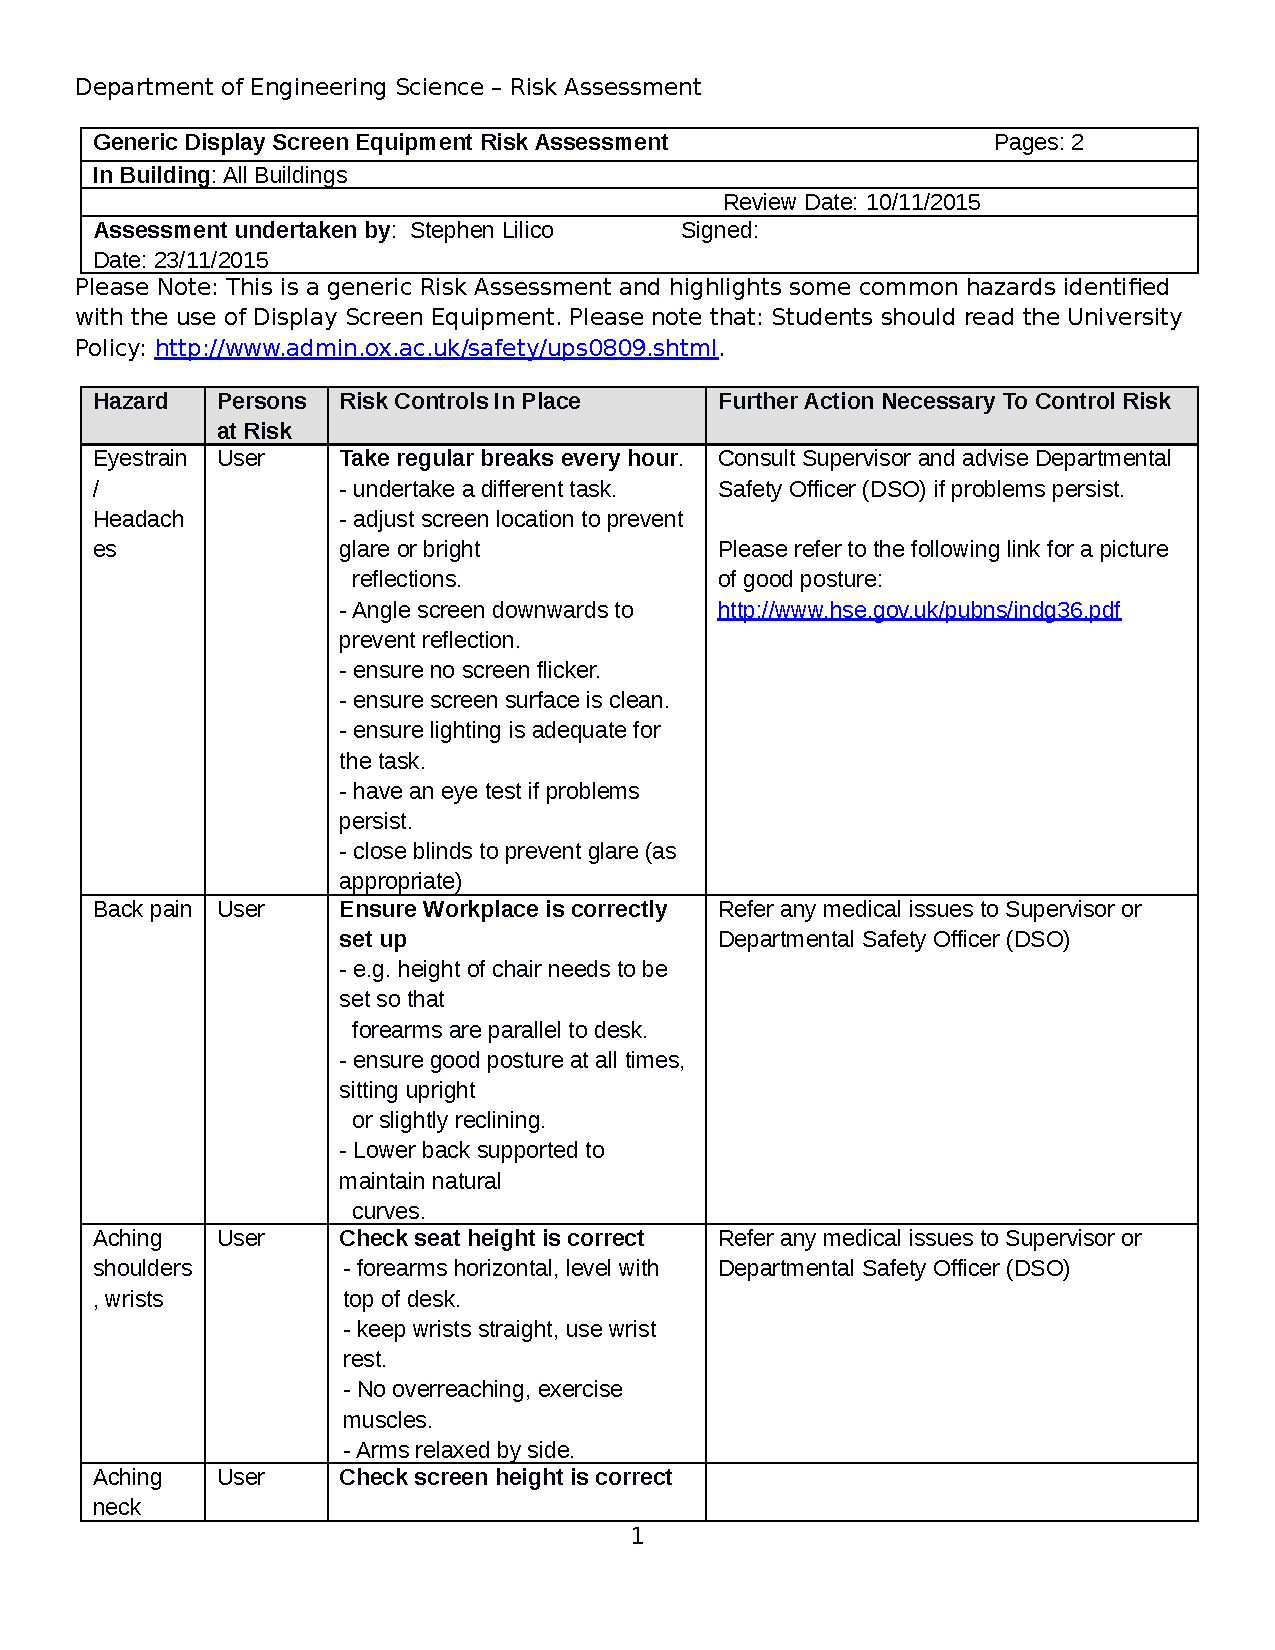
\includepdf[pages=-]{Risk_Assessment.pdf}


\section{Explaination of Code}
%this section details how the codebase works.

%do I even want to explain how the magic codebase works? - depends on space - probably? - it explains where all those hours went
\subsection{Summary of code for the Magic the Gathering agent}
The agent to play M:tG was also written in Java, which isn't ideal for optimisation, but was necessary because the emulator being used was written in Java. The neural networks library found did in fact have a c based back end and GPU implementation, though that turned out not to be the performance bottleneck anyway. The neural networks library was called neuralnetworks, found at https://github.com/ivan-vasilev/neuralnetworks. The emulator used is called forge, found at http://www.slightlymagic.net/wiki/Forge. The full code for this agent can be found at https://github.com/thesilencelies/LearnForge. 

There were several adjustments to the overall infrastructure of the emulator to allow the additional option of a learned-ai player, rather than just human or the hard coded ai, which needed to be kept so that is could be used to train the learning agent. Asides from those, all the additional materials can be found in the module titled learnedai. This uses entities titled Q-cards to store the assessment of each card, then combines them together into a matrix that can be fed to the neural network that assesses play states. The elements that model the future states and choose the highest scoring actions already existed, and were largely left as is, with the main adjustment being the replacement of the heuristic score system with the neural network.
The neural network is preserved because it is a static entity, and it was manoeuvred around the memory leak by regularly saving and loading the network, though that did delete the saved experiences from its experience replay.

\subsection{Code for the Function Optimiser}
%explain what they do as well - space doesn't seem to be too tight right now
The whole system is based on the implementation of Recurrent Visual Attention from the torch blog\cite{Torch:RVA}. It is written in lua using the Torch nn libraries, and additionally depends on the dpnn and rnn packages. All of the files can be found in the package rl-optim, though the init file will need modifying. It is formed as an extension to the package dp.

The following sections detail the exact behaviour and interface of each of the additional Torch objects created for this project. Everything has been coded so that it can be ran in a batched manner.

\subsubsection{FunctionData}
This object is a dataSource for the dpnn experiment. It contains a function that takes an input of some parameters and a coordinate of the same dimension and returns a scalar. This function can be accessed by calling \emph{getFunction()} It defines a series of parameters and calculates the minimum value for the function given those parameters using the algorithm defined in figure~\ref{alg:functiongen}. These are used as the inputs and targets for the experiment, the targets being necessary to calculate the reward. Unlike with standard dataSources, the data is only created at runtime, to a quantity specified by ``trainDataSize'' and ``testDataSize'' parameters.

\subsubsection{FunctionInput}
This is an NN module which takes a reference to a function at its creation. This function should take a set of parameters and a coordinate of the same dimension as the parameters as an input and return a scalar value. It also requires the normalisation constant being used to be given to it, so that it can normalise the output of the function.

 When \emph{updateOutput} is called, the expected inputs are the batch of function parameters, the new coordinate to check, and its previous output for this batch, or an empty tensor if this is the first time. It runs the given coordinates through the function it was given at initialisation, then it returns a tensor containing the minimum value received so far from the function, the coordinate that was input to the minimum value, the last coordinate checked, and the value it received for it.

When \emph{updateGradInput} is called it returns two tensors, one for the parameters, which is an empty matrix because the parameters are hidden from the rest of the model, and one for the location, which is the section of the gradient given to it that corresponded to the last location checked.

It has no internal parameters, so its effects are unchanged by the training.
\subsubsection{RLFeedback}
This is an observer from dpnn that calculates the total reward the agent received across the task and the agent's accuracy. These parameters are useful both for analysis and to enable early stopping. It has to be told whether or not to use log rewards on initialisation, and otherwise the behaviour is standard.

\subsubsection{OptimReward}%whats the correct name for this?
This function observes the output of the whole network, calculates the reward, subtracts the baseline and transmits the reward to the REINFORCE modules.

More specifically, this is a Criterion which takes as additional inputs the network being used (so that it can transmit the reward to it), the dimensionality of the function being explored (so that it can return tensors of the correct size), the normalisation constant being used, so that the targets can be normalised correctly, and whether to give log rewards and/or rewards on every step.

When \emph{updateOutput} is called,  it compares the output of the agent with the target and calculates the reward that it should receive.

When \emph{updatedGradInput} is called, it checks its inputs for a second input that is the baseline reward, then reduces the rewards by that value before transmitting them back to the agent by calling \emph{reinforce} on the module. The returned gradient is also the rewards so that the baseline reward can be learned.

\subsubsection{reinforceEveryStep}
A modification of ReinforceNormal from dpnn, This receives the reward received by the agent not only as if it stopped at the last step, but as if it had stopped after each step. Then it creates the gradient for each step based on that step's rewards. To do this, it has to receive a call from the recursor telling it which step it is at using the function \emph{declareStepNo(stepNo.)}. In the forwards direction, this module adds Gaussian noise to its input if it is training, but not if it is testing.

\subsubsection{RecurrentFunctionOptim}
This module is a recurrent wrapper that handles the way the data is passed across the network, based upon RecurrentAttention from the rnn package. It takes as inputs on instantiation the recurrent network that estimates the internal state (self.rnn), the network that estimates the next location based on the internal state (self.action) and the module that handles the function calculation along with some parameters (self.minvalmod). It runs the algorithm for a fixed number of steps and then returns the concatenation of all the outputs of the function module.

More specifically, at each forwards step it asks self.action for the next location to check based on the current internal state of self.rnn, passes that value through self.minvalmod, then feeds the output from that into self.rnn to produce a new internal state. This is repeated until it runs out of steps, and the final output is the concatenation of all of the outputs from self.minvalmod, to allow for everystep or other unusual reward schemes.

On the backwards pass it handles the back-propagation through time for all of its elements and the updates for their parameters.

\subsubsection{EqualSearch, PatternSearch and AmoebaSearch}
All of these objects are designed to produce the same type of output as RecurrentFunctionOptim, using the same number of limited calls to self.minvalmod, but instead of using internal neural networks to decide what location to check next, they use a hard coded algorithm to choose the next location. With EqualSearch it divides the search space into even sections and essentially ignores the output of self.minvalmod. PatternSearch maintains a centre coordinate, which it then checks around a fixed distance in each dimension, before moving  the centre to the new lowest observed value, or reduces the search distance if no new lowest value is observed. The amoeba search attempts to implement the simplex algorithm, though it is a little more complex as the simplex algorithm often wants to make multiple function calls per step, which means that often the steps of the simplex algorithm are spread across several steps that the agent takes.


\subsubsection{ApprenticedRFO}
This module is based on RecurrentFunctionOptim, but it first implements an example based gradient descent training - teaching the modules to attempt to replicate the output of a pattern search. It has two additional function calls beyond the standard module function calls - \emph{beFree()} and \emph{backToSchool()} which turn this "apprenticed" behaviour on and off.

Whilst running the apprenticed mode, in addition to the standard forwards pass from RecurrentFunctionOptim, it also produces a separate internal value called tutor, which is the equivalent results that would be produced by a pattern search agent were they to start at the same location as the agent under training, which is calculated using the same code as that ran in PatternSearch. Then, as long as the apprenticed behaviour is on, the gradient given to the agent isn't based upon the reward received (although the early stopping is), but instead on the difference between its output and the tutors for that step. In order to achieve this, a slightly modified form of ReinforceNormal was made that had the additional function \emph{enableReinforce(bool)} which told it whether or not to add noise and produce a gradient based on the reward, or simply pass through its inputs and gradients.

When not running the apprenticed mode, it is nearly identical to RecurrentFunctionOptim with the exception that it has a randomised starting location.

\subsubsection{DetRFO}
This module takes the same inputs as RecurrentFunctionOptim, plus a state generation (self.Qstate) and value-from-state-action (self.Qact) network for the critic. It implements an actor critic approach to the learning problem, along with a deterministic policy gradient, following the algorithms laid out in the paper on continuous control using the deterministic policy gradient\cite{lillicrap2015continuous}, which are explained in section~\ref{sec:detrfo}. It expects its function reinforce to be called by some criterion telling it what reward it has received.

Upon initialisation, it creates copies of self.action, self.Qstate and self.Qact to be the target networks. These networks do not have their parameters updated using the standard learning rules, rather they are updated to track the values from the originals using the update step \begin{equation}
\theta' \gets \tau \theta + (1 - \tau)\theta'
\end{equation} Where $\tau$ is very small.

\emph{updateOutput} is just like with RecurrentFunctionOptim. However, when \emph{updateGradInput} is called, first it saves the last experience, inputs, actions and rewards, into its experience replay memory, then it loads a new batch of experiences at random from the experience replay. Then it runs the critic networks on the experiences, and produces the gradient with which to update the actor networks. Then it produces the gradients for the critic to update, using a target generated from the bellman step for that experience, that is \begin{equation}
Q(s,a;\theta) = r + \gamma Q(s,a';\theta')
\end{equation} where $a'$ is the action produced by the target actor network for that state. Then it creates the internal state for that experience in the actor networks, before performing the back propagation for the actor, using the deterministic policy gradient.



\section{References}
\printbibliography[omitnumbers = false]
  
 %defined structure
 %Cover and Title Page: the project title, the author and their college affiliation
%should be prominently displayed, both on the front cover and on the first page.
%Your candidate number must not be included.
% Acknowledgements should be made of sources of help and finance. Helpful people appreciate gratitude.
% Abstract: a summary of the project, not longer than one page in length. This is best written last.
% Contents page giving page numbers of the main sections and sub-sections of the report.
% Sectional structure: for example
%1. Introduction
%1.1 What the project is about
%1.2 How the report is organised
%1.3 Who did what (if more than one author)
%2. Literature Review
%3. Technical section
%2
%4. Technical section ....
%n. Conclusions
%n.1 Summary, recapitulating what was achieved
%n.2 Recommendations for future work
%n+1. References
%Appendices
\end{document}

